\documentclass[a4paper, english]{article}

% Language setting
\usepackage[english]{babel}
\usepackage[version=4]{mhchem} % for chemical reactions 
% Set page size and margins
\usepackage[a4paper,top=2cm,bottom=2cm,left=3cm,right=3cm,marginparwidth=1.75cm]{geometry}
\usepackage{caption}
\usepackage{subcaption}
\usepackage{booktabs}
\usepackage{xcolor}
\usepackage{acronym}
%no blue acros 
% adjust colour of acronyms
\makeatletter
\AtBeginDocument{%
  \renewcommand*{\AC@hyperlink}[2]{%
    \begingroup
      \hypersetup{hidelinks}%
      \hyperlink{#1}{#2}%
    \endgroup
  }%
}
\makeatother

\usepackage{listings}
\lstdefinestyle{PyStyle}{
    commentstyle=\color{olive},
    keywordstyle=\color{magenta},
    numberstyle=\tiny\color{gray},
    stringstyle=\color{purple},
    basicstyle=\footnotesize,
    breakatwhitespace=false,         
    breaklines=true,                 
    captionpos=b,                    
    keepspaces=true,                 
    numbers=left,                    
    numbersep=5pt,                  
    showspaces=false,                
    showstringspaces=false,
    showtabs=false,                  
    tabsize=2,
    language=python
}

% Useful packages
\usepackage{amsmath}
\usepackage{graphicx}
\usepackage{wrapfig}
\usepackage[colorlinks=true, allcolors=blue]{hyperref}
\usepackage[capitalize]{cleveref}
\usepackage{csquotes}
\usepackage[iso]{isodate}
\usepackage[backend=biber]{biblatex}

\usepackage{titling} % for cooler titlepages 

\bibliography{refs.bib} % Entries are in the refs.bib file

\title{\textit{PMA Space Science and Technology M. Sc.} \\ \vspace{1cm}Project Report \\ \vspace{1cm} \textbf{\huge Automated detection of Urban Heat Islands using remote sensing data}\\ \vspace{1.2cm} }

\author{Linus Andrae (6015384)}
\date{\today}

\begin{document}
\begin{titlingpage} %This starts the title page
\pagenumbering{Alph}
\thispagestyle{empty} 
\begin{center}
\begin{large}
  \textit{University Bremen}\\
\end{large}
\vspace{4cm} %You can control the vertical distance
\begin{large} 
\textbf{\thetitle} 
\end{large}
\theauthor\\
\thedate\\
\vspace{13cm} %Put the distance you need.


\includegraphics[width=0.3\textwidth]{img/res/uniLogoIUP.png}
\hspace{4cm}

\includegraphics[width=0.3\textwidth]{img/res/logo_ohb_digital.png}

\end{center}
\end{titlingpage}
\pagenumbering{arabic}

\newpage
\begin{abstract}
\noindent
Urban Heat Islands (\acp{UHI}) pose a growing health risk by exacerbating heat stress for residents of urban areas. 
Due to the increased prevalence of extreme weather events and heat waves and as a cause for higher energy consumption, \acp{UHI} become more relevant as a topic for city planners and policy makers to consider.
Identification of areas most impacted or at risk require a data backed tool set to aid urban planning. 
This study presents a comprehensive pipeline developed using Python to automate the processing and analysis of Landsat 7,8 and 9 remote sensing imagery.
The pipeline facilitates the generation of Normalized Difference Vegetation Index (NDVI) and heat maps, running statistical analysis of factors known to create \acp{UHI} of a provided area of interest, serving as a robust toolset for the investigation and detection of \acp{UHI}.
The methodology employed leverages the spectral characteristics of Landsat data to provide high-resolution insights into temperature variations within urban areas as well as statistical analysis of the composition of the identified Urban Heat Islands.
The ultimate aim is to offer actionable guidance to city planners and developers for the mitigation of \acp{UHI}, by classification of \acp{UHI} on different scales.
At the current implementation level the pipeline is able to detect \acp{UHI} from level one brightness temperature and the statistical analysis indicate a strong correlation between land cover types and heat island intensity, affirming the utility of the pipeline in urban climate studies.
%To analyse and identify Urban Heat Islands using remote sensing imagery
\end{abstract}

\newpage
\tableofcontents
\listoffigures
\listoftables
\section*{Acronyms}
\begin{acronym}
  \acro{USGS}{United States Geological Survey}
  \acro{LST}{Land Surface Temperature}
  \acro{LULC}{Land Use/ Land Cover}
  \acro{UHI}[UHI]{Urban Heat Island}
  \acro{NDVI}{Normalized Differential Vegetation Index}
  \acro{NIR}{Near Infrared}
  \acro{OSM}{Open Street Map}
  \acro{TOA}{Top of Atmosphere}
\end{acronym}
\newpage

\section{Introduction}
    \subsection{Background}
   \section{Background}
\subsection{Urban Heat Islands}
The phenomenon of \acp{UHI} has been studied for the past 30 years. 
Due to increase in global temperature as well as increased occurrence of extreme weather and periods of heatwaves, this phenomenon will likely increase in intensity and will also occur in cities at higher latitudes~\cite{Sachindra2016}\cite[p.~904]{Wilby2008}.
\acp{UHI} are a spacial phenomenon that occurs on different scales and intensities, this makes observation using remote sensing data a good and widely used approach~\cite{Weng2003}.\\
\acp{UHI} are distinguished into surface and atmospheric \acp{UHI}.
Within this context we will only investigate surface \acp{UHI}. 
Surface \acp{UHI} are areas of higher surface temperatures within urban areas compared to rural areas due to the materials used and heat from mobility, electrical appliances, heating and cooling as well as less vegetation and higher sealed surfaces that reduce surface water availability\cite[pp. 7-12]{EPA2008}. 
The surface \acp{UHI} are longer term phenomenon that are most intense in summer. 
Atmospheric \acp{UHI} are more dependent on weather and local topology and are in part a side effect of the slower cooling of the city air due to the higher thermal capacity and wind obstruction.
This phenomenon is not investigated by this work, since the air temperature can not be directly observed by remote sensing data.
%Under certain conditions the increased temperature will form a hot air pocket, that will trap the head and reduce airflow from and to the area. \\
The main factors in forming urban heat islands is the thermal storage capacity of materials used in urban areas like concrete, asphalt and steel, that have a high heat capacity and heat up quickly during the day and emit the stored thermal energy as sensible heat with a delay (eg.~during the night)\cite{Ramamurthy2014}. 
High surface sealing and lack of vegetation reduce surface water availability and diminish evaporation and the cooling effect of latent heat causing more thermal energy to be available as sensible heat. %todo source (sailor?  or first source)
Another factor is the heat produced by human activity such as industrial processes and combustion engines.
As a consequence of higher temperatures, active cooling devices are more frequently used for buildings and vehicles. 
The emitted thermal energy of these heat pumps further increases the surrounding temperature, reinforcing the effect.
\\
There are multiple adverse effects and possible mitigation techniques for the mitigation and reduction of urban heat islands have been studied extensively since the 1970s\cite{Nichol1994}\cite{Stewart2011}. % list studies.  
Advective cooling can be observed when the temperature gradient generated airflow from the cooler surrounding areas towards the hot areas within the city, cooling it down\cite{HaegerEugensson1999}. \\
Urban areas with no close water body (generating sea breezes as well as latent heat transport) and with lower average wind speed are more likely to be affected by urban heat islands\cite{Ramamurthy2017}. 
Higher temperatures due to \acp{UHI} cause stress to animals and humans increasing health risk due to heat stroke and increased surface level ozone concentration\cite{Santamouris2020}.
\subsection{Land Surface Temperature}
Land surface temperature is the temperature at which an object emits infrared radiation according to plank's law\cite{Liang2020}. 
Using remote sensing methods this quantity can not be directly observed since the satellite is observing \ac{TOA} brightness temperature. 
This temperature can be transformed to a \ac{LST} using atmospheric correction and correction for the emissivity of the ground.
The conversion factor is data source dependent and can be found in \cref{sec:lstcalc}.

    \subsection{Research Question}
    \subsection{Methodology}
    \subsection{Structure of the Thesis}

\section*{Acknowledgements}

\section{Theoretical Framework}
    \subsection{Definitions}
    \subsection{Indices}
Many different indices are used for analysis of images or parameters in remote sensing, atmospheric physics and meteorology.
The following sections introduce the indices that where used to analyse the \glspl{UHI} within this work. 
\subsubsection{NDVI}
\textit{The following section is a slightly reworked version of a section from the pre-thesis master project~\cite{andrae2023}}\\ 
%
\noindent
\begin{figure}[!htbp]
    \centering
    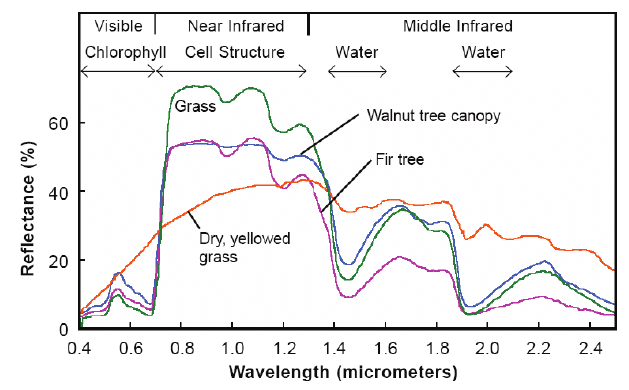
\includegraphics[width=0.5\textwidth]{img/Reflectance-spectra-of-different-types-of-green-vegetation-compared-to-a-spectral.png}
    \caption{Absorption spectrum of green vegetation \autocite[P. 5]{Smith2012}\label{fig:absorbtionVeg}}
\end{figure}
The \gls{NDVI} is an widely used index using the difference of the red and near infrared bands to determine the amount of green vegetation. 
\begin{equation}
    NDVI = \frac{Red-NIR}{Red+NIR}
    \label{equ:ndvi}
\end{equation}
For Landsat 8 and 9 data, channel 4 (red $640\ \text{nm} - 670\ \text{nm}$) and channel 5 (near infrared $850\ \text{nm} - 880\ \text{nm}$) where used.
As shown in \cref{fig:absorbtionVeg} healthy plants reflect near infrared and there is a sharp rise in reflectance between the two used channels at around $700\ \text{nm}$. 
%
This index is used for emissivity estimation for Land Surface Temperature calculation see \cref{equ:toa}, correlation with heat islands (since there is a negative correlation between those two values, due to the latent heat of evaporation reducing surface temperature at higher vegetation areas).
\begin{figure}[!htbp]
    \centering
    \begin{subfigure}{0.45\textwidth}
    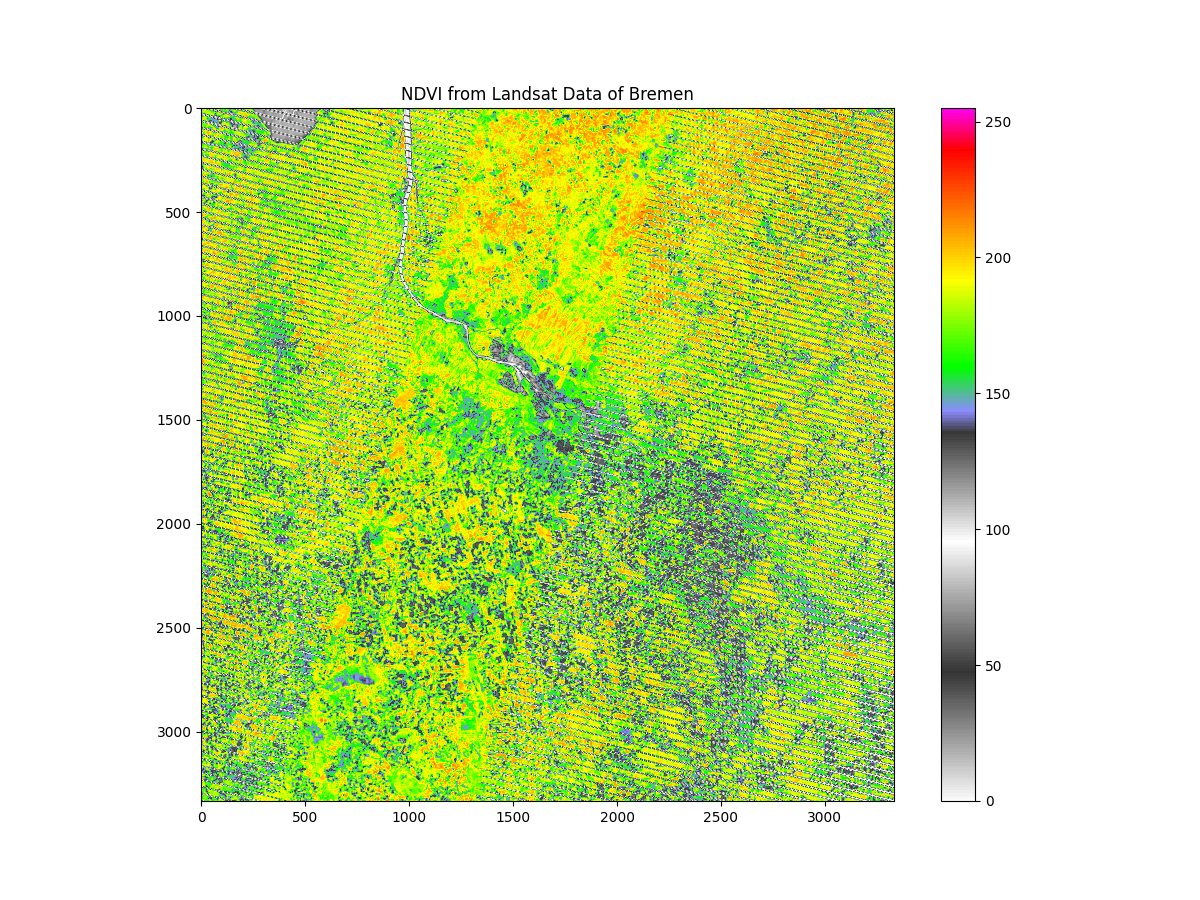
\includegraphics[width=\textwidth]{img/NDVI_LE07_L1TP_196023_20190723_20200825_02_T1__Bremen.png}
    \subcaption{NDVI of Bremen (Bands 5 and 6) using Landsat 7 data on 2019--07--23}
    \end{subfigure}
    \begin{subfigure}{0.45\textwidth}
    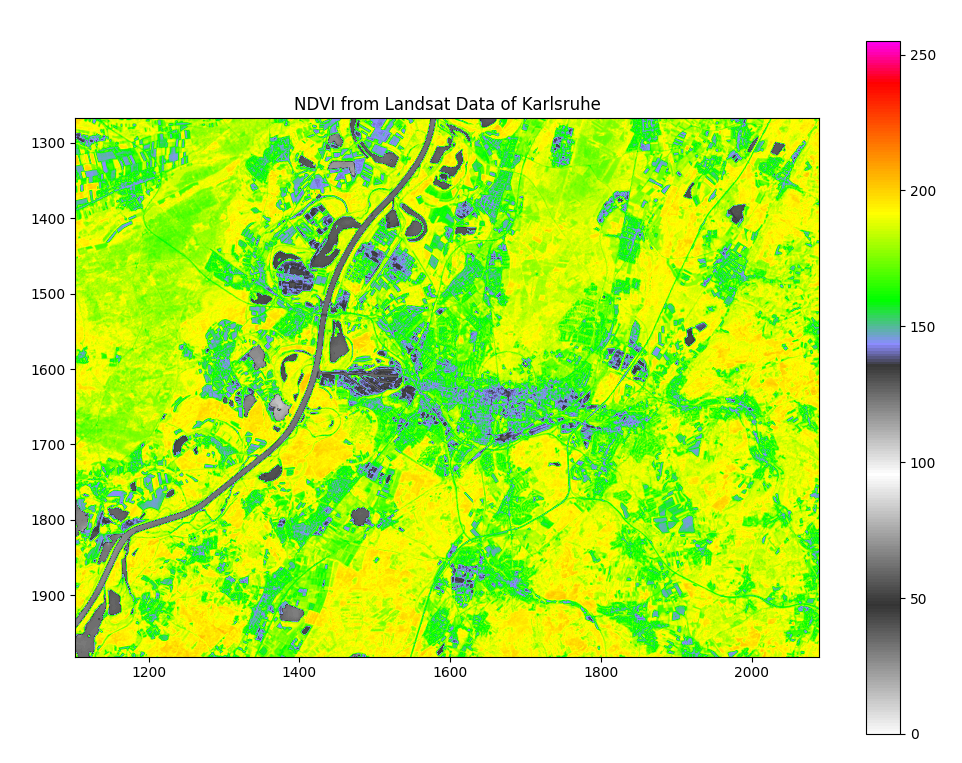
\includegraphics[width=\textwidth]{img/KarlsruheNDVI_Landsat8.png} 
    \subcaption{NDVI of Karlruhe (Bands 4 and 5) using Landsat 8 data on 2023--06--07}
    \end{subfigure}
    \caption{NDVI Images from the different satellites\label{fig:ndvi}}
\end{figure}
%\subsubsection{NDVI Colormap}\label{sec:colormap}
%When using a classical heat map with a color gradient from colder to warmer colors or a diverging color map (see \cref{fig:ndviPhoenixAzBad}), details of the image get lost and it is hard to distinguish plant heath, build up and vegetated areas and the difference between small \gls{NDVI} changes.
%To aid an intuitive understanding a specially created colormap can be used. 
%The color map was adapted for use in python from work of \texttt{public lab}\cite{ndviCmap} where it was developed in an attempt to create color-blind friendly \gls{NDVI} color maps.
%Values below 0.2 are areas with no vegetation.
%The color map used in \cref{fig:ndviPhoenixAz} uses a gradient of gray with a ``black-white-black
%white'' transition to allow higher dynamic range for non vegetation areas.
%For areas with an \gls{NDVI} $<$ 0.2 blue is used. Green values are low or unhealthy green vegetation or mixed use pixels. 
%Orange and red values correspond to thicker vegetation e.g.~forests, parks or green fields. 
%%
%Comparing \cref{fig:ndviPhoenixAz}  and \cref{fig:ndviPhoenixAzBad} where most of the desert surrounding the city has no green vegetation and the parts covered in vegetation can be clearly distinguished from the arid desert regions.
%Still the surface roughness can be seen quite well due to the gray scale gradient in the $<$ 0.2 \gls{NDVI} range.  
%%
%\begin{figure}[htbp]
% \centering
%    \begin{subfigure}{0.46\textwidth}
%    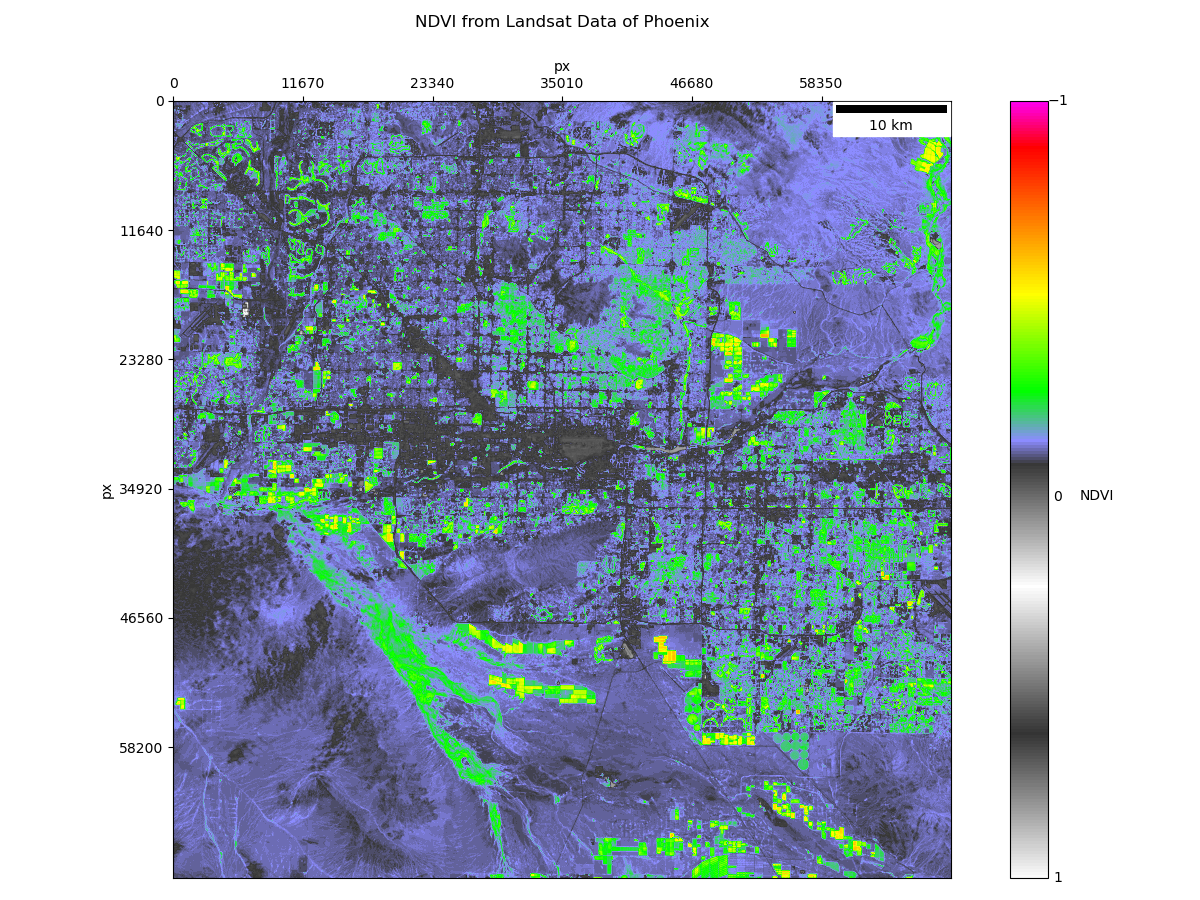
\includegraphics[width=\textwidth]{img/NDVI from Landsat Data of Phoenix.png} 
%    \subcaption{NDVI Image of Phoenix with the  VGYRM color map\label{fig:ndviPhoenixAz}}
%    \end{subfigure}
%    \begin{subfigure}{0.46\textwidth}
%    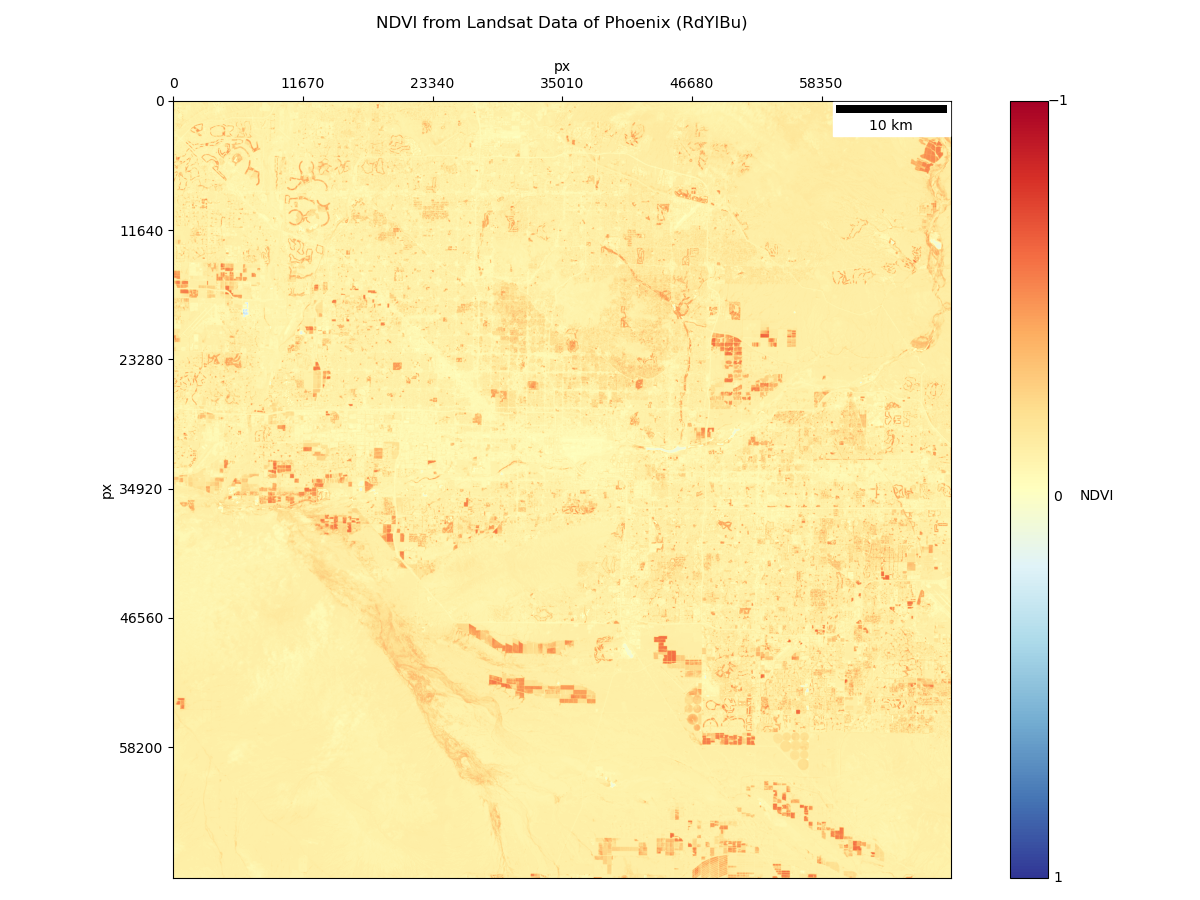
\includegraphics[width=\textwidth]{img/NDVI from Landsat Data of Phoenix (RdYlBu).png} 
%    \subcaption{NDVI Image of Phoenix with a RdYlBu gradient color map\label{fig:ndviPhoenixAzBad}}
%    \end{subfigure}
%    \caption{Different color maps used show the better ability to differentiate between green vegetation and desert and buildings within Phoenix\label{fig:ndvicomp}}
%\end{figure}

    \subsection{Models and Theories}

\section{Comparable Definition of Urban Heat Islands}
    \subsection{Introduction}
    \subsection{Analysis}
    \subsection{Conclusions}

\section{Impact of Climate Change on UHIs}
    \subsection{Introduction}
    \subsection{Analysis}
    \subsection{Conclusions}

\section{Impact of Land Use Land Cover Changes on UHIs}
    \subsection{Introduction}
    \subsection{Analysis}
    \subsection{Conclusions}

\section{Simulation and Modeling of UHIs}
    \subsection{Introduction}
    \subsection{Analysis}
    \subsection{Conclusions}

\section{Discussion}
    \subsection{Synthesis of Findings}
    \subsection{Implications}

\section{Conclusion}
    \subsection{Summary}
    \subsection{Future Work}

\section{Appendix}
    \subsection{Data}
    \subsection{Code}

\section{Objectives}
The goal of the project was to investigate \acp{UHI} using remote sensing data. 
To find out what steps are needed to detect \acp{UHI} in different climate and seasonal conditions multiple cities where investigated. 
The cities where investigated in different time frames and different data sources where used.  
The cities that where selected where: 
\begin{itemize}
    \item Bremen  due to the possibility to locally verify land use on ground
    \item Karlsruhe, this city developed a heat action plan and has an interesting geology 
    \item Speyer lies in one of the hottest areas in Germany with more then 40 days per year with over 25 \textdegree C that is in a similar geographical area as Karlsruhe and allows comparison of urban and geographic features due to close distance between cities
\end{itemize}
%
%
Other questions that this work wanted to answer where: \\
\begin{itemize}
  \item How strong is the correlation between \acp{UHI} and vegetation? 
  \item Can a simple estimation of the land surface temperature be enough to detect \acp{UHI} compared to the Level two products of the satellite data. 
    %\item How big are the error margins in \ac{LST} calculation for \acp{UHI} detection using remote sensing data and different algorithm. 
\end{itemize}
%data pipeline to create maps of \acp{UHI} in areas 
%- surface classification based on remote sensing data correlated with 2nd and 3rd sources (kataster/ OSM) 
%- \ac{UHI} "cores" identification 
\section{Scope}
Part of this effort was the planning, development and verification of software that \acp{UHI} can be detected using remote sensing data automatically. 
The data processing of the pipeline that was developed was verified and statistical analysis about land usage, vegetation and temperature data where conducted. 
The developed software is used as parts of the toolset for further analysis of \acp{UHI} as part of a master thesis. 
%\section{Literature Review}


\section{Methodology}
The process used in this project used a data driven approach to answer the questions above. 
First the available remote sensing data sources where evaluated and the Landsat satellites where selected due to availability, usage in similar research towards \acp{UHI}\cite{Weng2004}\cite{Weng2003}\cite{Jumari2023} where selected.
Based on %previous research and 
the possibilities to do local on site verification Bremen was chosen as a first area of investigation. 
From the remote sensing data the \ac{NDVI} and \ac{LST} where calculated and surface type classification was done. 
Based on the derived data statistical analysis where made to investigate the correlation between \ac{NDVI}, surface types and \ac{LST}. 
The same approach was done for Landsat 7 and Landsat 8 images. 
Urban heat islands where detected using statistical analysis of the derived \ac{LST} data. 
\subsection{Data Quality}
The Landsat 7 Data has a resolution of 30m~x~30m for all channels but the thermal channels, the thermal infrared channels have 60m~x~60m per pixel\cite{Landsat7Specs} with 8 bit color depth. 
In Landsat 7  Images only scenes can be properly used where the targeted area of interest lies in the center region of the swath, since starting in march 2003 the scan line correction onboard the ETM+ instrument failed and up to 22\% of the scene can not be used\cite{Landsat7Specs}.
For Landsat 8 Data the resolution of the reflective channels are identical, the thermal channels have a 100m~x~100m resolution with a higher grayscale color range per pixel of 12-bit\cite{Landsat8Specs}.
Errors due to cloud shadows\cite[p.14]{EROASC2013} where eliminated by using images with no clouds for the areas of interest.
\newpage
\section{Implementation}
The application that was created uses python and the luigi module to allow building scalable pipelines with automated dependency management. 
This allows to change a single stage in the pipeline % and brake everything... 
and allow automatic inclusion of switched dependencies or additional process steps that can be configured by passing parameters to prior steps within the pipeline. 
\begin{wrapfigure}{r}{0.58\textwidth}
    \centering
    \raisebox{0pt}[\dimexpr\height-0.8\baselineskip\relax]{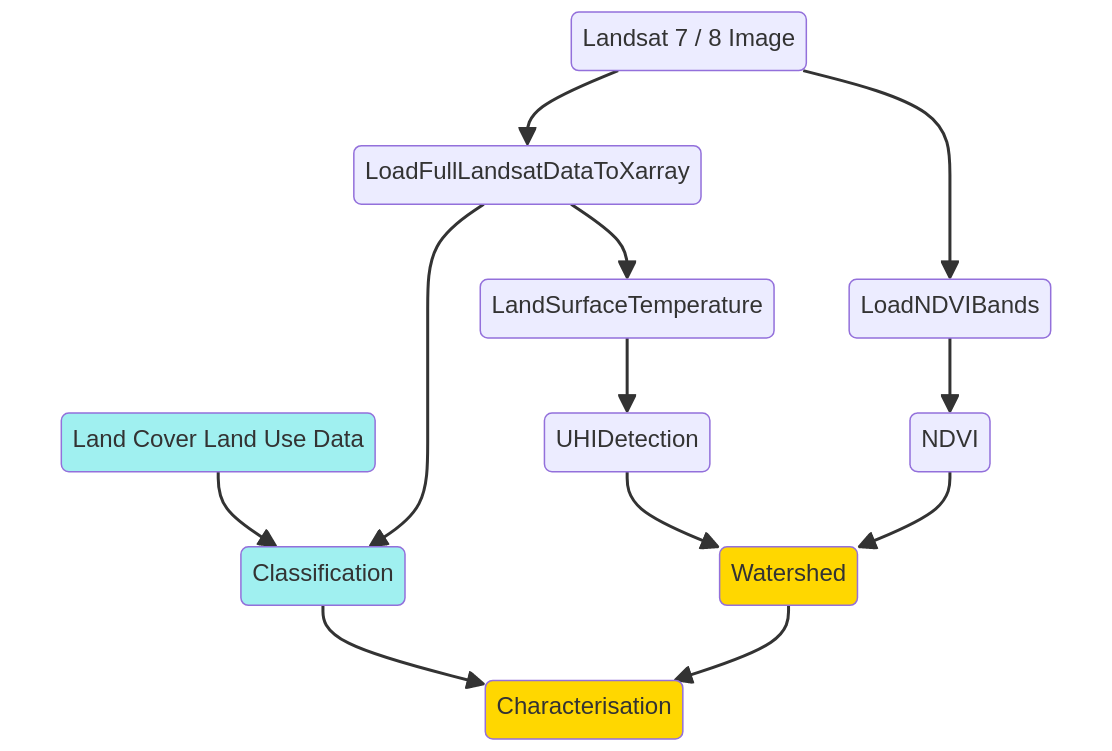
\includegraphics[width=0.56\textwidth]{img/DiagPipeline}}
    \caption{Pipeline stages for data processing\label{fig:pipeline}}
    \vspace{-2em}
\end{wrapfigure}
To allow quick adaption and partly automated analysis different software modules where created. 
This part will give an overview over the implemented parts, the overall workings and outlook for possible additions and shortcomings of the currently implemented software. 
\subsection{Pipeline design}
The python software is designed as a data pipeline with different steps that automatically trigger previous requirements when run using the \texttt{Luigi} module\cite{swLuigi}.
A startup script initiates the pipeline by calling the last stage as a luigi task. Each tasks will in turn start the required previous stages it depends on for execution, building up a requirement graph that will start the end nodes once all requirements where found. 
Once a stage or task is completed the next step is triggered and run. 
In case of an error the pipeline execution will be stopped.
\Cref{fig:pipeline} shows the software data flow, purple steps are part of the \ac{UHI} detection and statistical analysis and purely based on Landsat data. Blue steps are related to \ac{LULC} classification.
Yellow steps are future additions and not implemented yet. 
In the following section each pipeline stage will explained for the steps in turquoise and purple shown in \cref{fig:pipeline}.
% Detailed look at the code, libraries used, software architecture, etc.
\subsection{Loading an Image} 
The images in GEOTIFF format can be loaded by the pipeline as single bands (\texttt{LoadBands}, \texttt{LoadNDVIBands}) or as a full set of Bands (\texttt{LoadFullLandsatDataToXarray}). 
Bands are loaded as numpy arrays and in the full set load function stored inside an xarray data structure where each band data is named individually by band name, to ease usage independent of the data source band enumeration.
Between pipeline steps the data is stored in a temporary zipped numpy binary format \texttt{npz}, this allows multiple steps to work with the same output.
%
\subsection{Preprocessing}
The preprocessing of the images is done by cropping the image to the area of interest by providing a center coordinate and the bounding box height and width in m (north-south and east-west sizes) 
The transformed image might be filtered if needed by a later pipeline stage. 
%The data for analysis is downloaded and placed into a folder, alternativly a pipline stage can be added to directly download a scene using the \ac{USGS} downloader API. 
%\begin{figure}[!htbp]
%    \centering
%\end{figure}
%Depending on the selected pipeline steps the source data can either be L1 or L1 and L2 data from Landsat 7, 8 or 9. 
\subsection{Land Surface Temperature Calculation}
\subsubsection{Calculation of the Landsat L2 LST}
The \ac{USGS} provides \ac{LST} data for Landsat 7,8 and 9 Thermal instruments\cite{EROASC2013}\cite{EROASC1999} online after around two weeks after data acquisition. 
The level two data set uses the top of the atmosphere temperature and calculates the \ac{LST} using atmospheric correction, correction for absorption and emissivity based on ASTER GED data set for radiation temperature.
%
\subsubsection{Estimation of the LST temperature based on Landsat L1 Data}\label{sec:lstcalc}
To check the functionality of the pipeline and create a possibility to create land surface temperature maps from raw data a estimation algorithm was implemented based on the Landsat level 1 data. It was correction for emissivity based on the \ac{NDVI}, this is not as accurate as the ASTER data but provides LST maps quickly and can be derived from a single image data set of the Landsat mission. 
The landsat intensity value can be converted to a  brightness temperature using \cref{equ:toa}(see \cite{usgsLSTLandsat})
\begin{equation}
    \begin{split}\label{equ:toa}
      L_{\lambda} &= M_L\cdot Q_{cal} + A_L \\
      BT_{TOA} &= \frac{K2}{\ln(\frac{K1}{L_{\lambda}} + 1)}
    \end{split}
\end{equation}
%
For the $L_{\lambda}$ the \ac{TOA} radiance is calculated from the $M_L$ parameter from the band meta data file and the additive rescaling factor that is also included in the meta data of the image. 
Where K1 and K2 are satellite dependent correction parameters and $L_{\lambda}$ is the observed brightness temperature at the satellite instrument. 
The resulting \ac{TOA} brightness temperature is then corrected using fixed factors based on the \ac{NDVI}. 
The conversion to \ac{LST} can be done using satellite dependent steps and the correction based on \ac{NDVI} are for Landsat 8  and for Landsat 7. %TODO shown in \cref{equ:lstL8}.
\begin{equation}\label{equ:lstL8}
  LST = \frac{T_{TOA}}{1+\frac{\epsilon\cdot T_{TOA}}{1.4388}}
\end{equation}
%
To approximate a proper emissivity correction the \cref{equ:emslstL8}\cite{Sobrino2004} is used.
\begin{equation}
\begin{split}\label{equ:emslstL8}
  \epsilon &= m \cdot P_v + n \\
  P_v &= \frac{NDVI-NDVI_{min}}{NDVI_{max}- NDVI_{min}}
\end{split}
\end{equation}
With $P_v$ beeing the vegetative fraction 
where $n$ and $m$ are correction factor for emissivity of partly vegetated areas.  
%
For \ac{NDVI} values below 0.2 the surface is assumed to be not populated by any green vegetation and the emissivity is taken from the red band\cite{Nichol1994}.
For \ac{NDVI} $>$ 0.5 the area of a pixel is assumed to be fully vegetation and the emmissivity can be assumed as 99\%\cite{Sobrino2004} and the values in between can be calculated by the above method with m and n taken from previous research as $m = 0.004$ and $n = 0.986$
~\cite[equ.~12a\&b]{Sobrino2004}.
%
In the following analysis the $BT_{TOA}$ is used without emissivity correction, to test and show that the raw data can be used to detect \glspl{UHI}. 
%The atmospheric influence and the material properties might 


%m per pixel. 
%A noticeable speciality of the Landsat data are the empty stripes at the image edges, these are caused by an error condition in the image scanner and cause empty pixels at the edges, degrading image quality for some targets.  
%
\subsection{Surface classification}
As basis for the statistical analysis and to classify the composition and formation of \acp{UHI} \ac{LULC} must be determined and differenciated, this was done using k-means as a pixel based clustering algorithm. 
%as well as machine learning to assign labels from a manually pretrained data set %todo do this in sw ;) 
The classification algorithm used blue, green, red and near infrared bands of the datasets to find pixel that have a similar composition.
By referencing the against \ac{OSM} land classification data%, land register data from the \textit{Bremen Geoinformation Zentrum} 
and local on site verification the classification results where verified.
An automatic pixel based comparison did not yield the desired results so a manual verification was done using the above mentioned resources. 
For future usage it would be suggested to use Sentinel-2  land cover or any other high resolution \ac{LULC} data set for verification.
For the \ac{OSM} verification the land usage types shown in \cref{tbl:types} of \ac{OSM} where used af the HeiGIT OSMLandUseLandCover project where used for manual verification (see \cref{fig:classification})
\begin{table}[!htbp]
    \centering
    \begin{tabular}{l l}
      \toprule
    \textbf{K-Means Classification} & \textbf{OSM tag} \\ \midrule
    Low density residential streets &  residential, commercial, religious, education, recreation\_ground \\ 
    Residential low vegetation & residential, commercial, religious, education\\ 
    Industy & construction, industrial, depot, port, railway, garages\\ 
    Industy Halls & industrial, depot \\ 
    Vegetation Agriculture & farmland, meadows\\ 
    Fields Meadows & farmland, meadows, grass, recreation\_ground\\ 
    Forests, trees \& dense vegetation & cemetery, trees, forest\\
    Water & water \\
    No Data & -- \\\bottomrule
    \end{tabular}
    \caption{The mapping of OSM Tags and KMeans surface classification types}
    \label{tbl:types}
\end{table}
%
\begin{figure}[!htbp]
    \centering
    \begin{subfigure}{0.58\textwidth}
    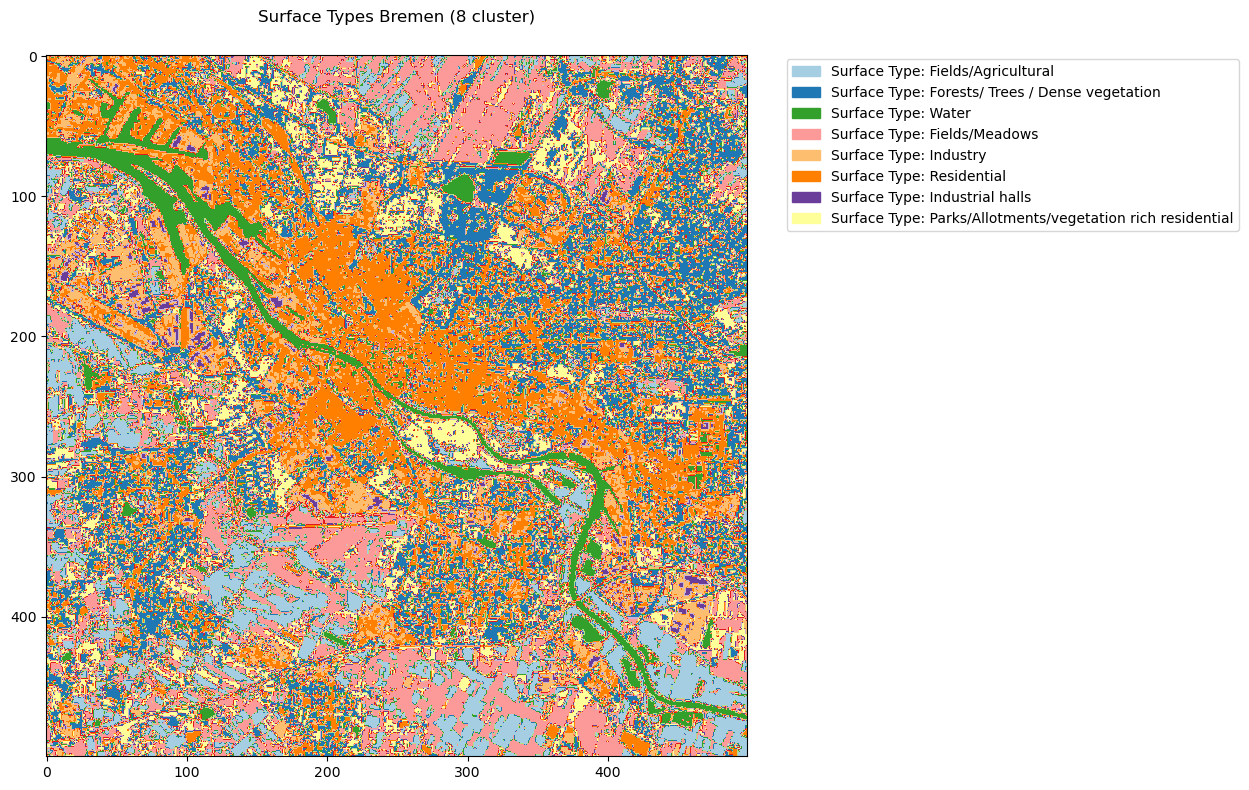
\includegraphics[width=\textwidth]{img/Surface Types Bremen (8 cluster).png}
      \subcaption{KMeans surface Types}
    \end{subfigure}
    \begin{subfigure}{0.40\textwidth}
    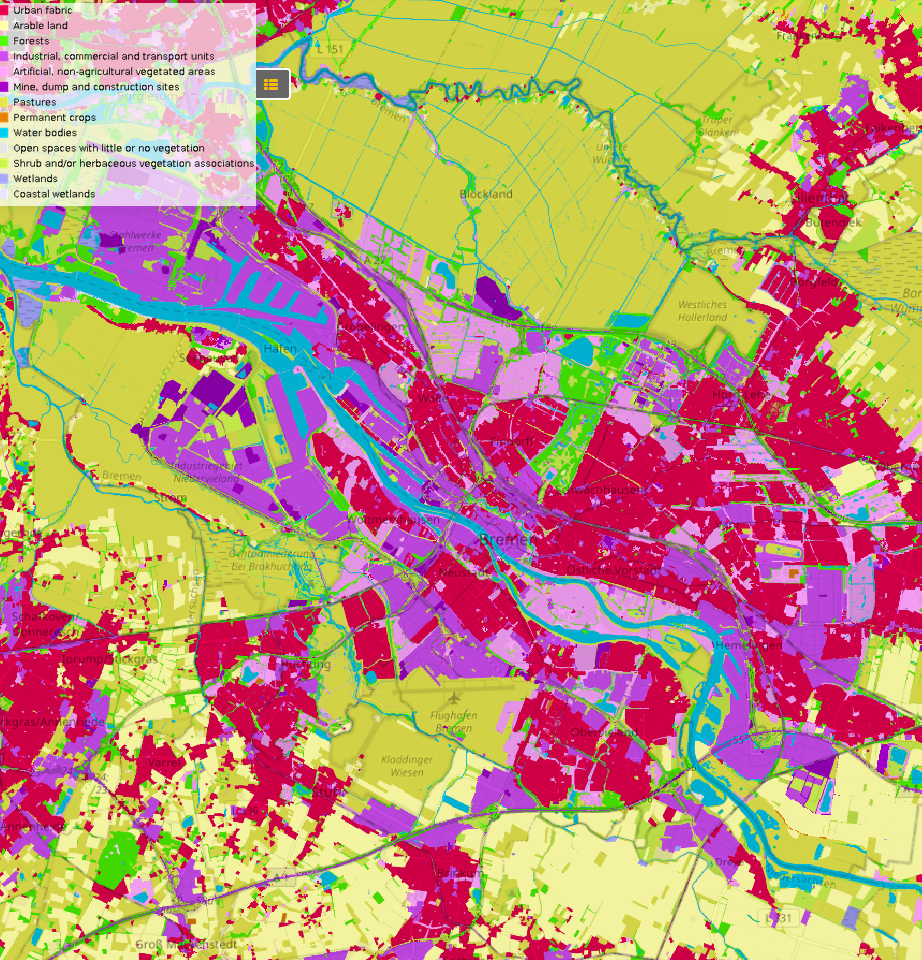
\includegraphics[width=0.95\textwidth]{img/OSMLandUseData.png}
      \subcaption{OSM Surface types (Image cutesy of OSMLanduseLandCover of HeiGIT\cite{Schultz2017})}
    \end{subfigure}
    \caption{Classification of the Bremen Land usage using K-Means \label{fig:classification}}
\end{figure}

\subsection{Detection of the Urban Heat Islands}\label{sec:uhiDetection}
To detect the \acp{UHI} from the \ac{LST} calculated before, a simple statistical threshold was applied. 
The temperature has to be by more then $2.5 \sigma$ higher then the average temperature of the image section, to be classified as a \ac{UHI}. 
The threshold of 2.8 was used to make results more comparable between cities. 
%The \ac{LST}, since the $\sigma$ was much smaller and the range of max and minimum temperature was lower compared to \ac{LST} estimations based on level 1 data, where a 3$\sigma$ threshold was used.
The usage of the mean of the whole area might cause a lower mean temperature if the shape of the urban area is ellipsoidal and surrounded by colder surfaces, this could be mitigated by either using a shape file to limit the area used for calculation or changing the threshold value for \ac{UHI} detection. 
Since city limits do not correspond to an immediate change in \ac{LULC} this was not done in the cities investigated here.
%
The \ac{LST} image where post processed to find all high heat areas and find and label connected high heat pixels to create contours of the significant higher temperature regions (shown in \cref{fig:UHIsKarlsruhe},\cref{fig:UHIsSpey} and \cref{fig:UHIsHB}). Areas smaller then 3 pixels where filtered out, since these likely correspond to single high heat or reflectivity pixels due to single roofs or other buildings, that did not cause a heating effect over a larger area.
/newpage
\begin{figure}[!p]
    \centering
    \begin{subfigure}{0.49\textwidth}
    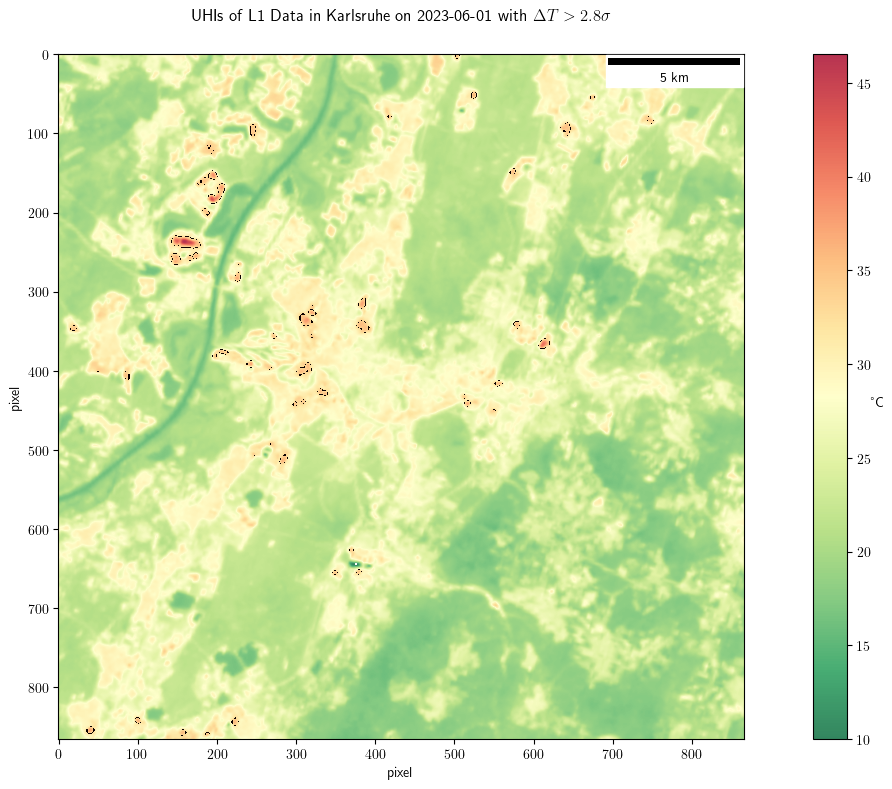
\includegraphics[width=\textwidth]{img/UHIL1Karlsruhe.png}
      \subcaption{UHI based on Level 1 Data}
    \end{subfigure}
    \begin{subfigure}{0.49\textwidth}
    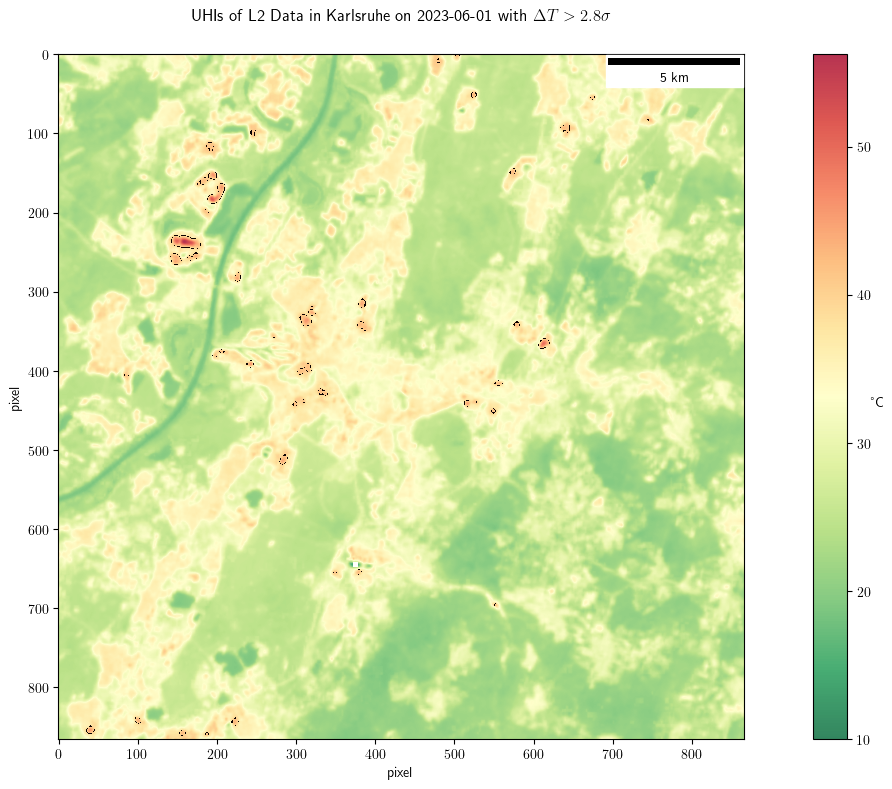
\includegraphics[width=\textwidth]{img/UHIL2Karlsruhe.png}
      \subcaption{UHI based on Level 2 Data}
    \end{subfigure}
    \caption{UHIs detected in Karlsruhe\label{fig:UHIsKarlsruhe} based on L1 and L2 Data}
\end{figure}
\begin{figure}[!htbp]
    \centering
    \begin{subfigure}{0.49\textwidth}
    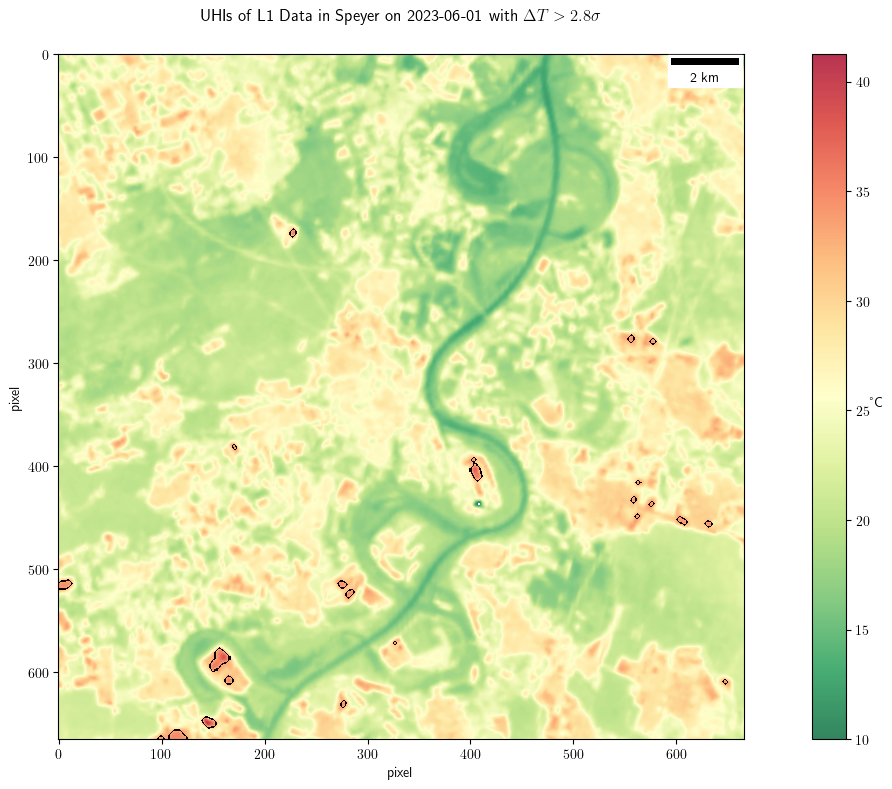
\includegraphics[width=\textwidth]{img/UHIL1Speyer.png}
      \subcaption{UHI based on Level 1 Data}
    \end{subfigure}
    \begin{subfigure}{0.49\textwidth}
    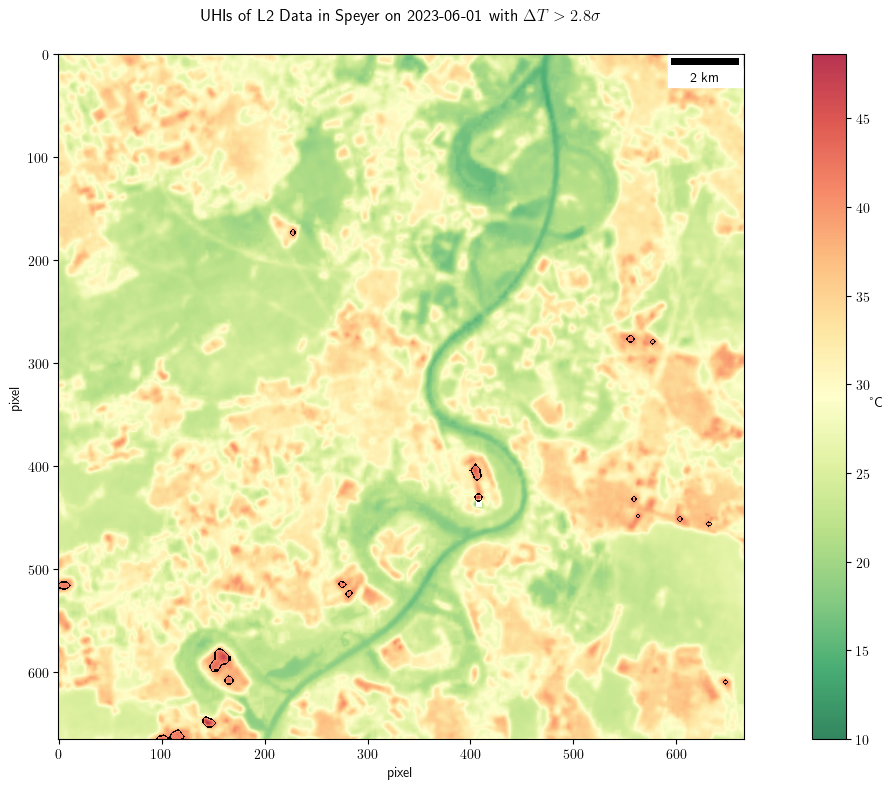
\includegraphics[width=\textwidth]{img/UHIL2Speyer.png}
      \subcaption{UHI based on Level 2 Data}
    \end{subfigure}
    \caption{UHIs detected in Speyer\label{fig:UHIsSpey} based on L1 and L2 Data}
\end{figure}
\begin{figure}[!htbp]
    \centering
    \begin{subfigure}{0.49\textwidth}
    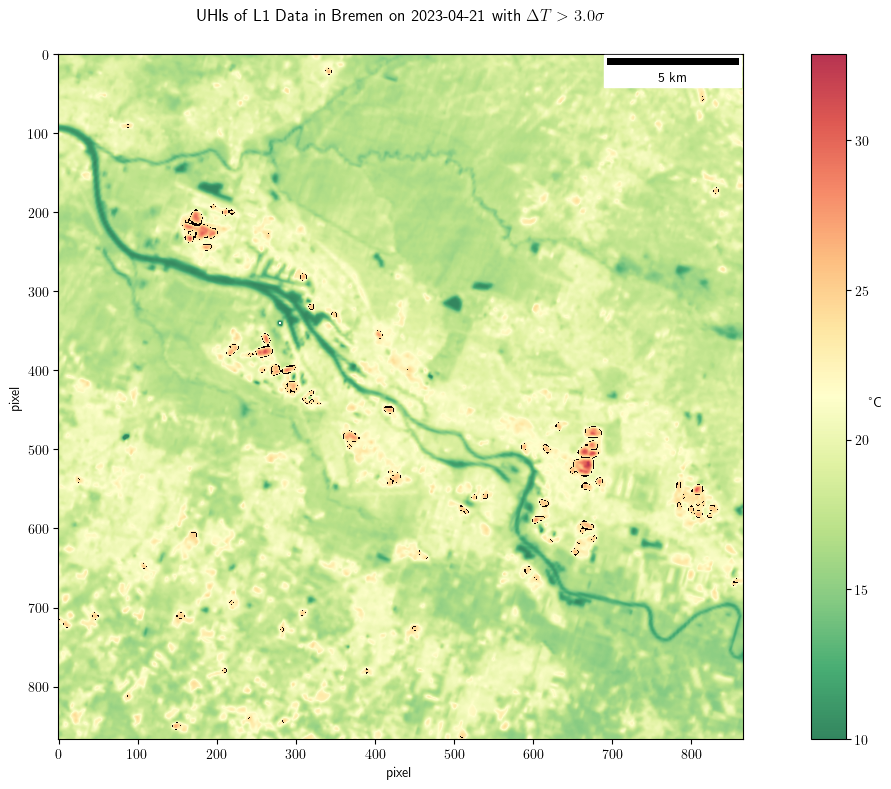
\includegraphics[width=\textwidth]{img/UHIL1HB.png}
      \subcaption{UHI based on Level 1 Data}
    \end{subfigure}
    \begin{subfigure}{0.49\textwidth}
    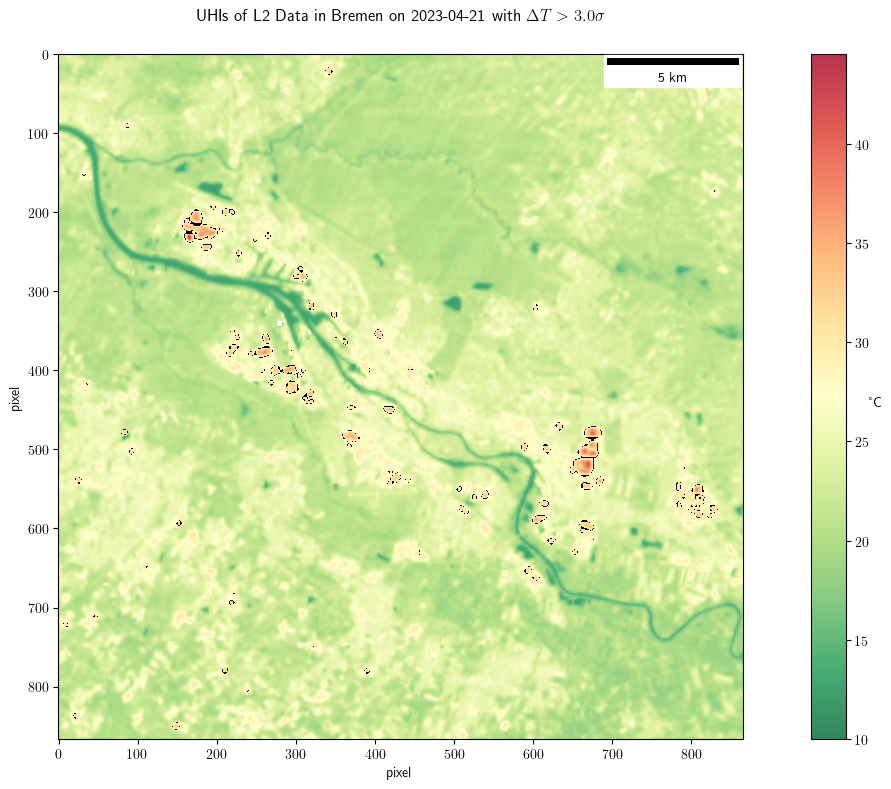
\includegraphics[width=\textwidth]{img/UHIL2HB.png}
      \subcaption{UHI based on Level 2 Data}
    \end{subfigure}
    \caption{UHIs detected in Bremen\label{fig:UHIsHB} based on L1 and L2 Data}
\end{figure}
\subsection{Further analysis steps (not yet implemented)}
After \acp{UHI} where detected further analysis could be added to the pipeline. 
A watershed analysis of the \acp{UHI} can be used to a dynamically vary the threshold what areas are affected by the \ac{UHI} from each center pixel to analyse scale effects of the \acp{UHI}. 
Another possible  addition would be to analyse the shape of the \ac{UHI} contour with different thresholds or at different seasons to investigate the influence of mean temperature, seasonal changes, city development and rising mean temperatures over time due to climate change on the \ac{UHI} effect. 
\newpage
\section{Analysis}\label{sec:analysis}
\subsection{Comparison of \ac{TOA} and L2 \ac{LST}}
\begin{wrapfigure}{r}{0.58\textwidth}
 \centering
    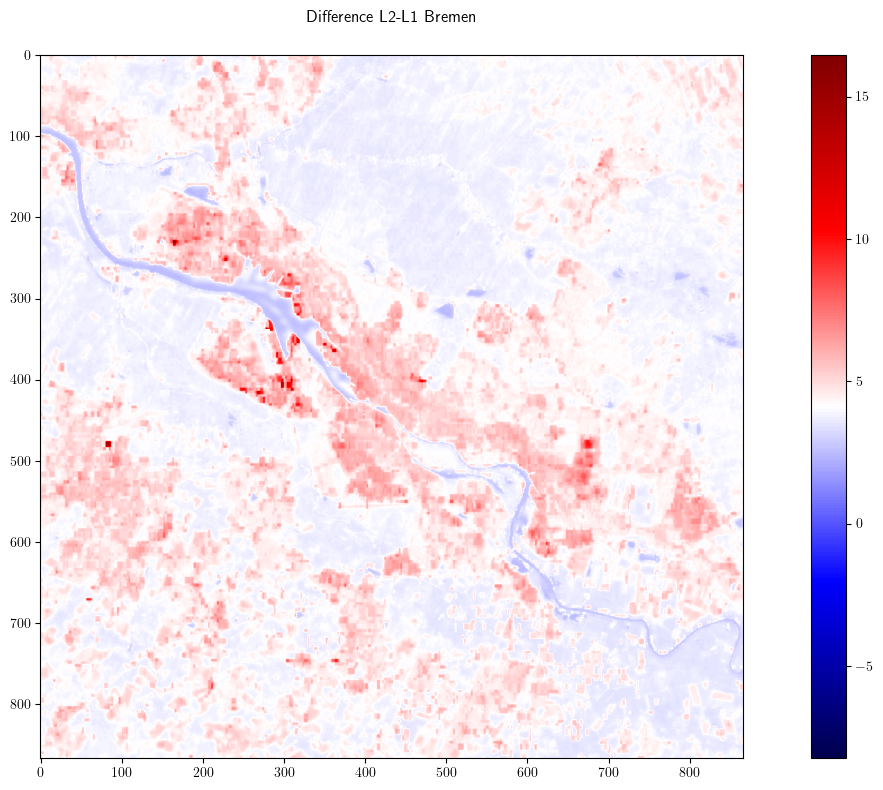
\includegraphics[width=0.5\textwidth]{img/Difference L2-L1.png} 
    \caption{Difference between L1 and L2 Data of Bremen\label{fig:t1t2diffHB}}
\end{wrapfigure}
Comparing the two data sets, a significant offset was seen between the L2 \ac{LST} and the \ac{TOA} from the L1 data (see \cref{fig:t1t2diffHB}).
%
The range of temperatures was more then 50\% bigger in the data that was not corrected for emissivity compared to the L2 data corrected by the USGS using the ASTER emissivity database. 
This suggests that emissivity correction is needed for high quality result when working with absolute temperatures. 
The uncorrected data does allow basic detection of \ac{UHI} since the relative temperatures are spread out more 
but the internal distribution doesn't change significantly (see the high correlation between the offset temperature data in \cref{fig:L1L2Bremen} -- \cref{fig:L1L2Spey}). \\
This allows the detection of \acp{UHI} based on level one data, while taking some under detection into account, due to atmospheric dampening.
%The temperature data was referenced with soil temperature measurements of the DWD station at Bremen Airport that measures soil temperature at 5 cm below the surface.
This allows to use Landsat L1 data for creating relative temperature maps that are able to detect urban heat island, since the UHI is a relative temperature effect. 
\begin{figure}[!htbp]
 \centering
    \begin{subfigure}{0.32\textwidth}
    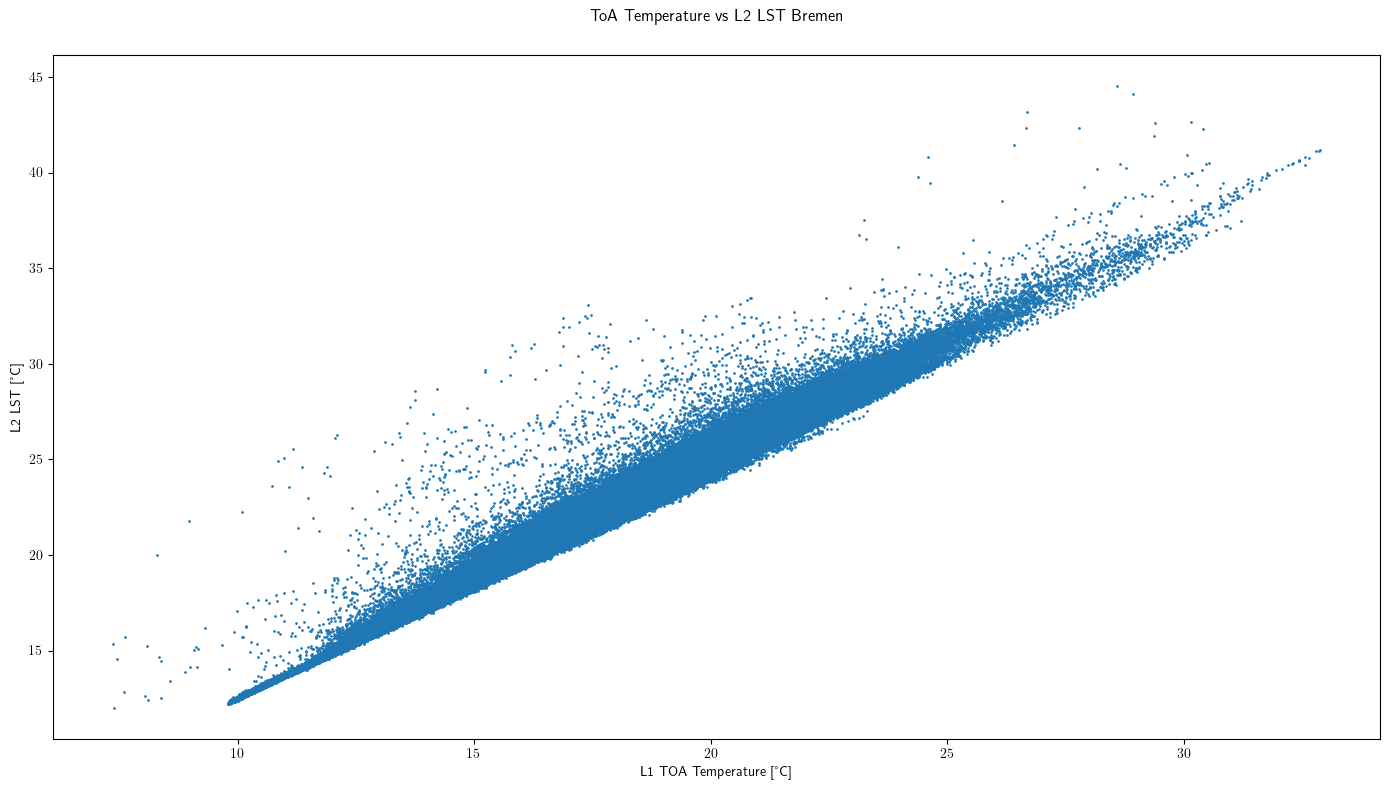
\includegraphics[width=\textwidth]{img/L1L2Bremen.png} 
      \subcaption{Bremen\label{fig:L1L2Bremen}}
    \end{subfigure}
    %
    \begin{subfigure}{0.32\textwidth}
    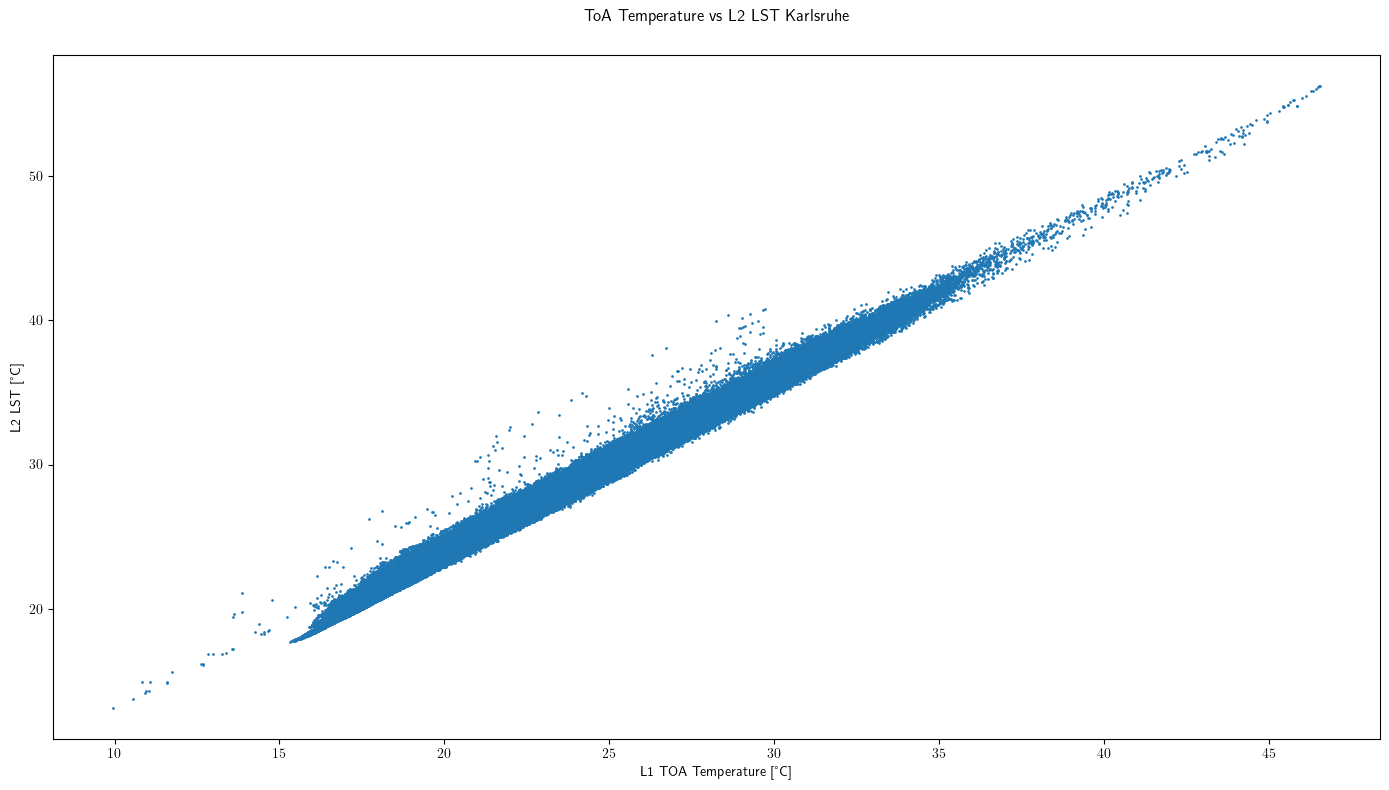
\includegraphics[width=\textwidth]{img/L1L2Karlsruhe.png} 
    \subcaption{Karlsruhe\label{fig:L1L2Karlsruhe}}
    \end{subfigure}
    %
    \begin{subfigure}{0.32\textwidth}
    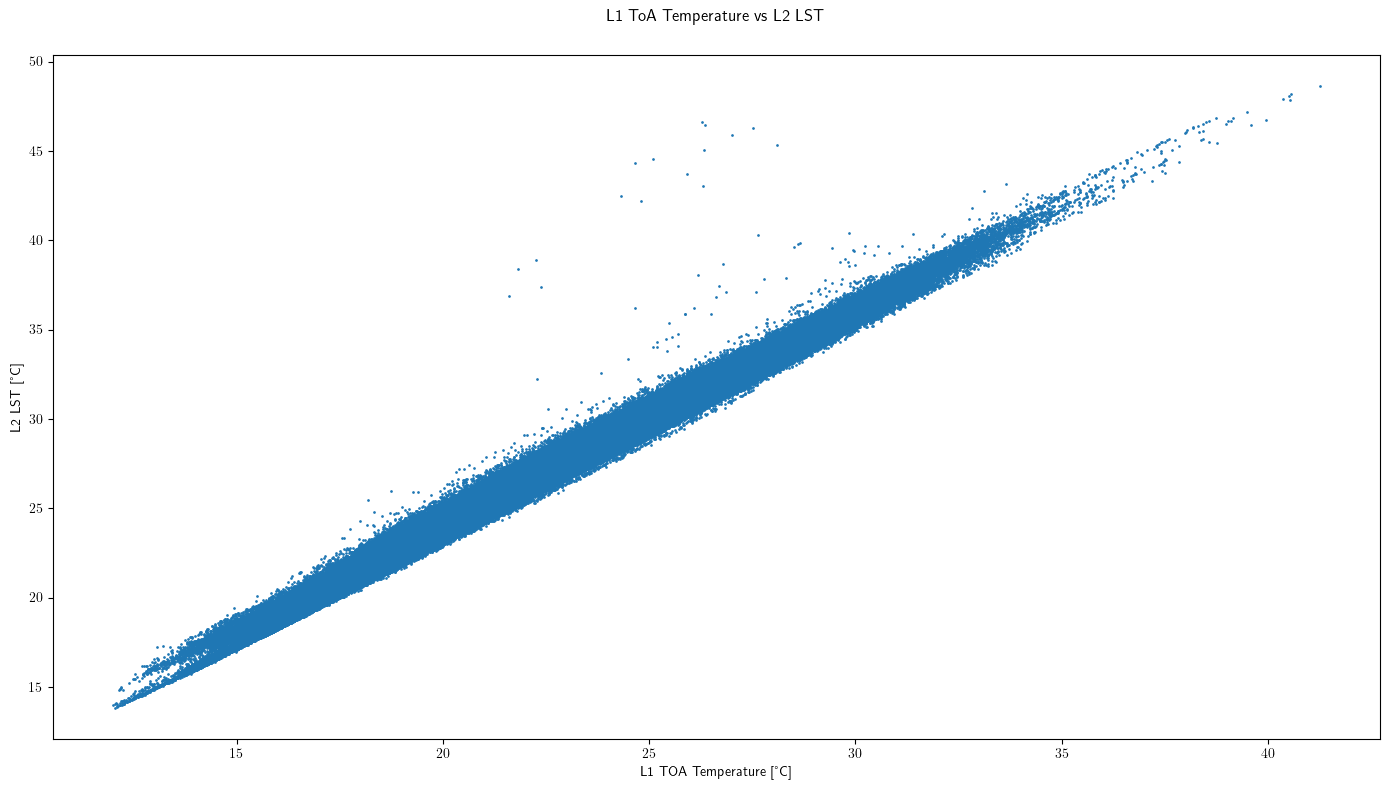
\includegraphics[width=\textwidth]{img/L1L2Speyer.png} 
    \subcaption{Speyer\label{fig:L1L2Spey}}
    \end{subfigure}
    %
    \caption{Correlation between the observed TOA and the L2 LST\label{fig:l1l2comp}} 
\end{figure}
For level two data an uncertainty value is given for each pixel. 
For the Bremen image with a range of 1.8 \textdegree to 9.5 \textdegree C with an RMS error of 2.62 \textdegree C, the whole temperature range was offset compared to the L1 data to higher temperatures (by 5.37 \textdegree C on average).
There where 41 pixels in three clusters with very high uncertainty values (above 7 \textdegree C), these where all located over industrialized areas and are likely caused by smoke plumes or the reflections of industry hall roofs. %TODO add image to appendix?
For Karlsruhe the maximum uncertainty for level two data was 7.98 \textdegree C the minimum 1.93 \textdegree C and the RMS uncertainty was 2.5 \textdegree C.
All 18 pixels with more then 7 \textdegree C uncertainty where located in two clusters over industrial areas.
For Speyer the maximum uncertainty for level two data was 6.11 \textdegree C the minimum 1.99 \textdegree C and the RMS uncertainty was 2.7 \textdegree C.
The highest degree of uncertainty was observed over the water surfaces, specifically over the river Rhine. 
\newpage
\subsection{UHI detection}
Using Landsat 7 and Landsat 8  data it was possible to identify urban heat islands in Bremen, Karlsruhe and Speyer using the level 1 and level 2 data products shown in \cref{fig:UHIsKarlsruhe},\cref{fig:UHIsSpey} and \cref{fig:UHIsHB}.
\\
A statistical analysis was done on the correlation between the \ac{LST} and the different land cover types as well as the \ac{NDVI} and the \ac{LST}.
The following data used the Landsat 8 Acquisition of Bremen from 2023--04--21 and the level 2 \ac{LST} data was used.
In \cref{fig:ndviVsLst} the \ac{LST} of each pixel is shown with the corresponding \ac{NDVI} value and the class for each pixel.
The Water pixels had a low \ac{NDVI} as to be expected and had the lowest temperatures within the image. 
%
\begin{figure}[!htbp]
    \centering
    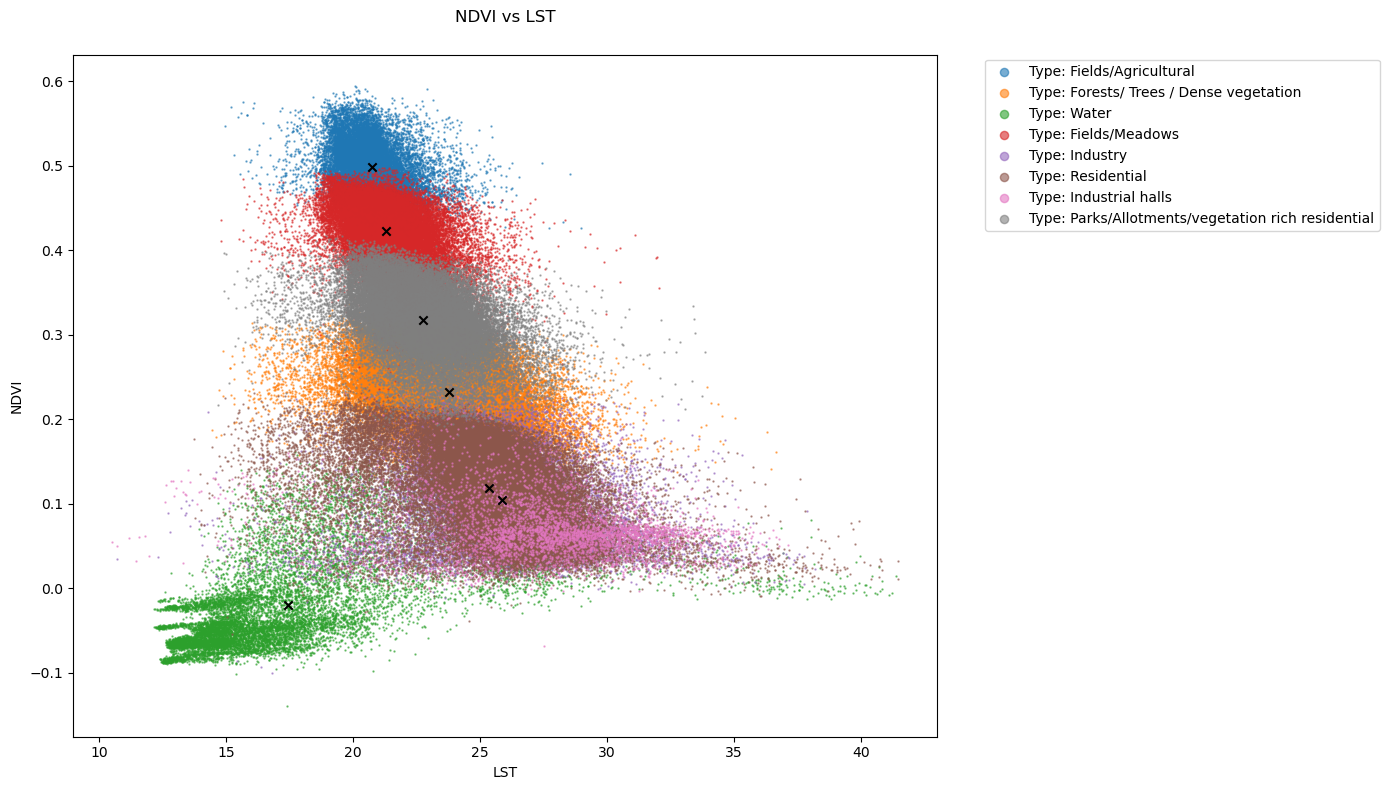
\includegraphics[width=0.97\textwidth]{img/NDVI vs LST.png}
    \caption{Land Surface Temperature versus \ac{NDVI} value\label{fig:ndviVsLst}}
\end{figure}
It can be seen that there is a strong correlation for all clusters except the water class between low temperatures and a high \ac{NDVI} and higher temperatures and low \ac{NDVI}. 
%
%The data also shows that the non vegetation classes have generally a smaller range of temperatures, that might be caused by neighbourhood effects, different building materials used or different emissivity of the surface material, since the data was not corrected for emissivity values before calculating the \ac{LST}.\\
%tODO regenerate ignoring 0 values
%\textit{TODO: Annotate that image or regenerate with different color for \ac{NDVI} classes to make it better understandable?}
%
%        Results and what they mean.
%        Could include code snippets, charts, graphs, etc.
The classes that where created using the kmeans algorithm and four bands show the distinction of classes in the amount of vegetation that is found within the pixels of each type in \cref{fig:ndviVsTypes} and for the distribution of \ac{LST} for each class in \cref{fig:scatterLstNDVI}.
As seen in the scatter plot (\cref{fig:clusters}) the clusters where mainly distributed within the near infrared band since the other bands have a very high correlation ($>0.95$ in the investigated images).
Since this channel is used for \ac{NDVI} creation, there is a high correlation between \ac{NDVI} and classification.
It can be seen that the highest brightness values are part of the industry halls that contains all metal roofed large buildings that reflect in all wavelengths. 
The other clusters are mainly distributed along the \ac{NIR} intensity values and then differ slightly within colors (e.g.~green intensity for different vegetation classes while the center of build up classes differ within the blue or red intensity).
%The 
\begin{figure}[!htbp]
    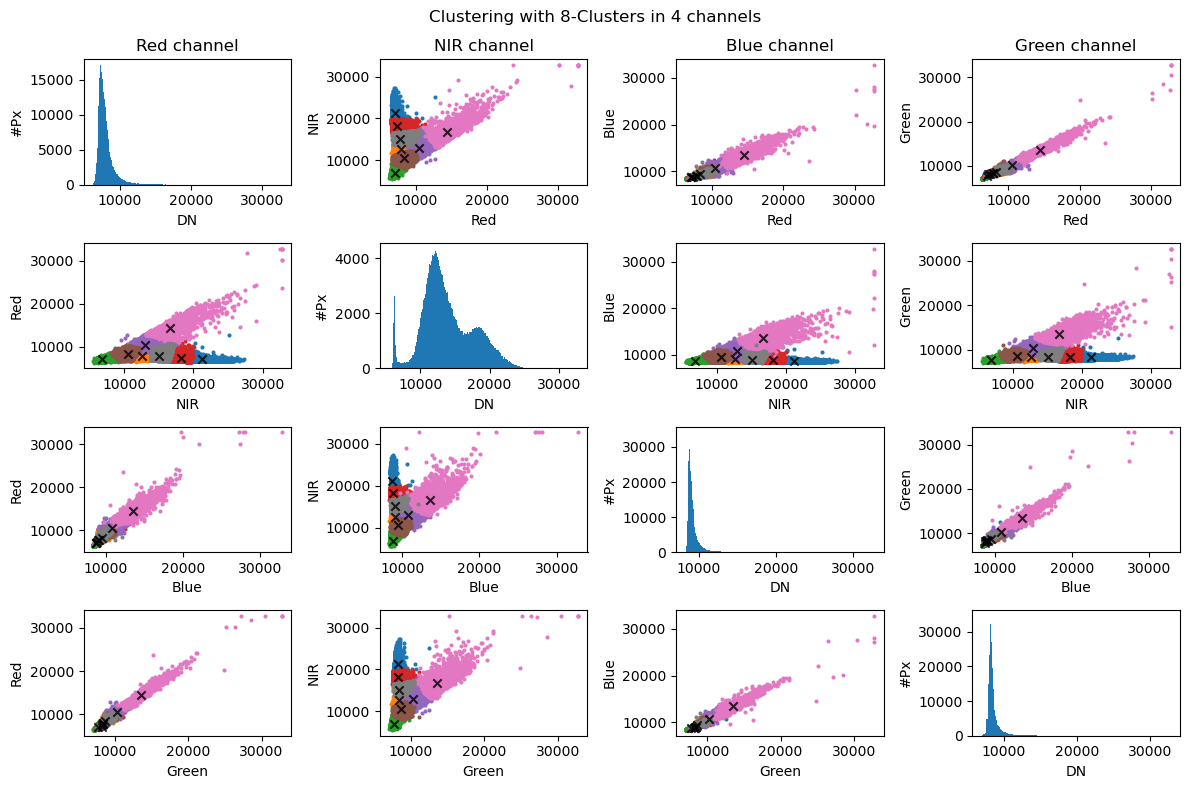
\includegraphics[width=\textwidth]{img/ScatterplotClustersAndHist.png}
    \caption{Results of the clustering and histograms on channel\label{fig:scatterLstNDVI}}
\end{figure}
%
\begin{figure}[!phtb]
    \centering
    \begin{subfigure}{\textwidth}
    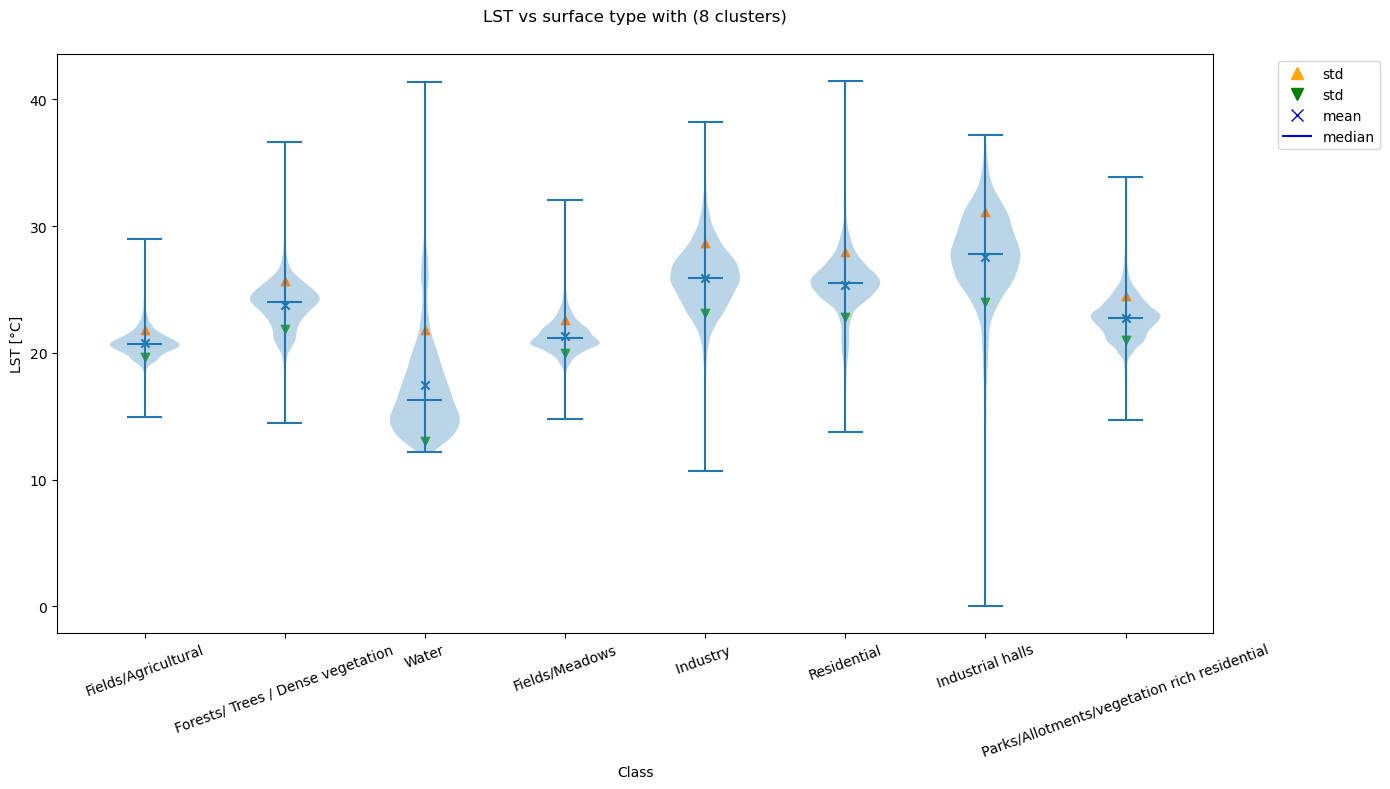
\includegraphics[width=\textwidth]{img/LST vs surface type with (8 clusters).png}
    \subcaption{Surface temperatures of the pixels within each class, with minimum maximum and internal distribution\label{fig:lstvsTypes}}
    \end{subfigure}
    \begin{subfigure}{\textwidth}
    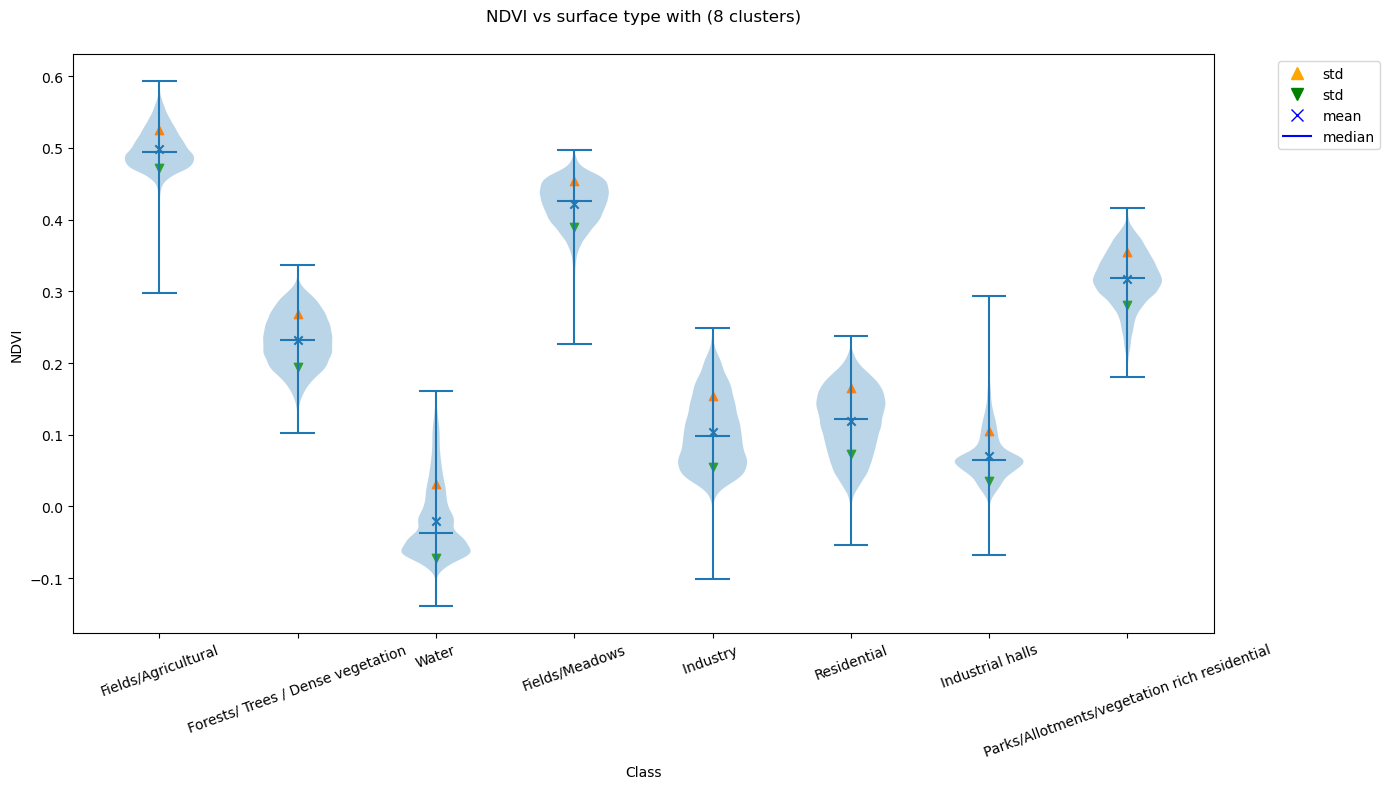
\includegraphics[width=\textwidth]{img/NDVI vs surface type with (8 clusters).png}
    \subcaption{\ac{NDVI} values of the pixels within each class\label{fig:ndviVsTypes}}
    \end{subfigure}
    \caption{\ac{LST} and \ac{NDVI} values of the pixels within the classes on a pixel based level\label{fig:clusters}}
\end{figure}
The \ac{LST} distribution between classes shows small dense clusters of temperatures near the mean temperature for all vegetation classes with low growing vegetation having the lowest spread of temperature. 
Build up land classes have a high temperature spread and higher mean and median temperatures. 
The 0 \textdegree C temperature value for the \textit{Industy halls} class is caused by four pixels with no data due to invalid data in the \ac{LST} dataset.
The very high spread temperature within the water class is in part explained by the temperature anomalies mentioned earlier and on the other hand by the different types of water bodies found within the image (small lakes, ditches and ponds as well as the river Weser). 
\newpage
\section{Results}
Using the Landsat satellite data allowed the calculation of the \ac{LST} for all investigated areas without emissivity correction with an offset of between 2 and 12 \textdegree C on average for the three investigated areas.
The level two correction for surface material emissivity does change the surface temperature values but not significantly change the temperature distribution.
%A small geometrical analysis showed that the \ac{
%After the investigation of different cities, urban heat islands where detected with the software. 
%TODO check if this is reasonable 
The average temperature of the selected areas and the maximum temperatures detected in the \acp{UHI} are shown in \cref{tbl:tempCities}
\begin{table}[!htbp]
    \centering
    \begin{tabular}{l l l l l}
      \toprule
      \textbf{City} & \textbf{Mean LST} & \textbf{$LST_{min}$[\textdegree~C]} &\textbf{$LST_{max}$[\textdegree~C]} & \#UHIs (threas.)\\ \midrule
% LS 7...
      %Bremen L1 (2019--07--23)&   27.52 ($\sigma = 2.7$) &14.7 & 46.26  & 164\\
      %Bremen L2 (2019--07--23)&   34.87 ($\sigma = 4.17$) &17.5 & 62.46  & 130\\
      %LS 8 
      Bremen L1 (2023--04--21)&  18.38  ($\sigma = 2.05$) &6.6 & 32.87 & 70 (3$\sigma$)\\ 
      Bremen L2 (2023--04--21)&   22.68 ($\sigma = 2.62$) &12.0 & 44.54  & 84(3$\sigma$)\\
      Karlruhe L1 (2023--06--01)& 23.48 ($\sigma = 3.83$) &9.32 & 46.54  & 86 (2.5$\sigma$)\\
      Karlruhe L2 (2023--06--01)& 27.91 ($\sigma = 4.81$) &13.15 & 56.25  & 74 (2.5$\sigma$)\\
      Speyer L1 (2023--06--01)&   22.94 ($\sigma = 3.88$) & 9.34 & 41.26  & 49 (2.5$\sigma$)\\
      Speyer L2 (2023--06--01)&   27.47 ($\sigma = 4.87$) &13.8 & 48.64  & 39 (2.5$\sigma$)\\
 & \\\bottomrule
    \end{tabular}
    \caption{Temperatures and \acp{UHI} observed in different Cities\label{tbl:tempCities}}
\end{table}
%
The statistical analysis was adapted for each city and can not be compared since the data was taken on different dates, the area of interest and shape of the cities are quite different and thus the mean temperatures and absolute thresholds are different. 
%
Comparing Karlsruhe and Speyer that have the same data set as baseline (both are within the same image captured on the same day by the Landsat 8 satellite).
It can be seen that there are more \acp{UHI} detected in Karlsruhe (the city is bigger and the selected Area of interest is as well) then in Speyer. 
The mean and 
Also the Karlsruhe area has a higher mean temperature and higher maximum temperature. 
In both cities the heat islands were located within industrial areas, low temperatures where within vegetated or near water areas.
\Cref{fig:UHIsHB} shows Bremen at the end of april where the local air temperature of that day was at around 19 \textdegree C (Source: Deutscher Wetterdienst Bremen airport station) at the time of recording. 
The biggest heat islands detected within the area are all located within industrialized parts of the city. 

%TODO maybe add in depth correlation here? 
%TODO add table with statistical data 
%\begin{figure}[!htbp]
%    \centering
%    \begin{subfigure}{\textwidth}
%    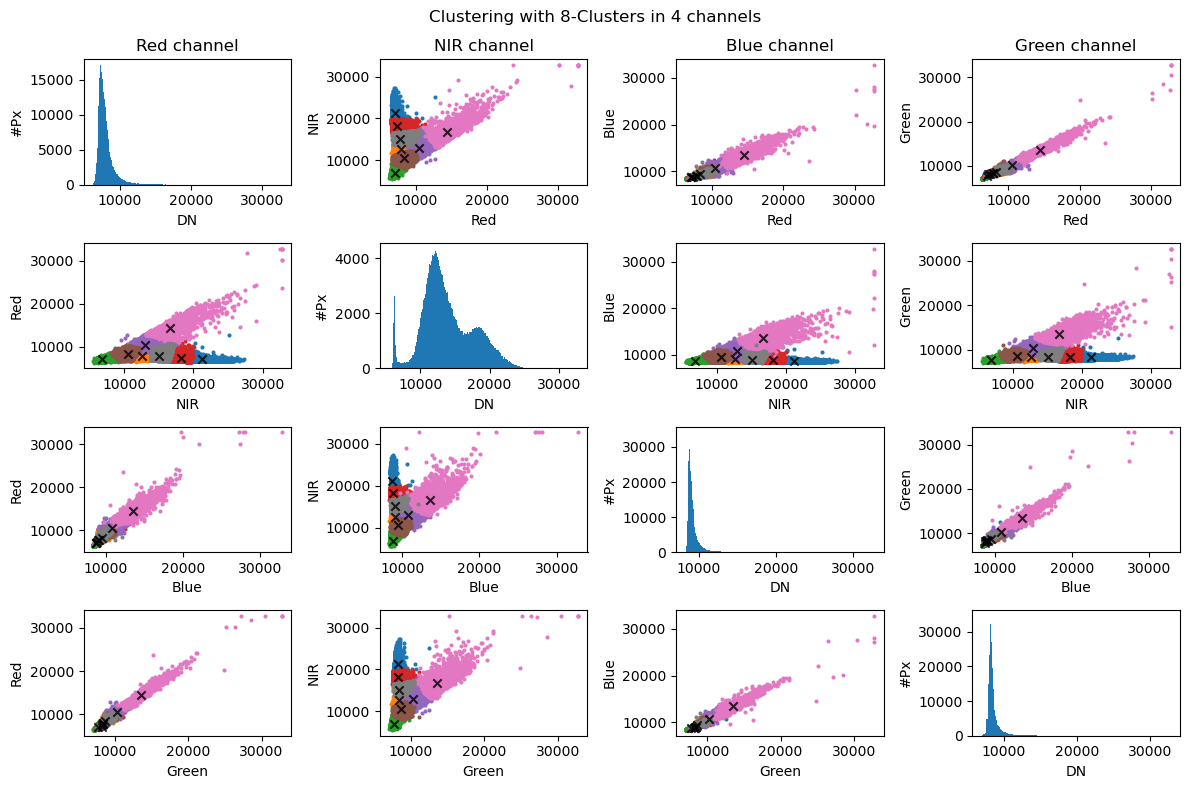
\includegraphics[width=\textwidth]{img/ScatterplotClustersAndHist.png}
%    \subcaption{Scatter plot of the different channel intensities\label{fig:scatter}}
%    \end{subfigure}
%    \begin{subfigure}{\textwidth}
%    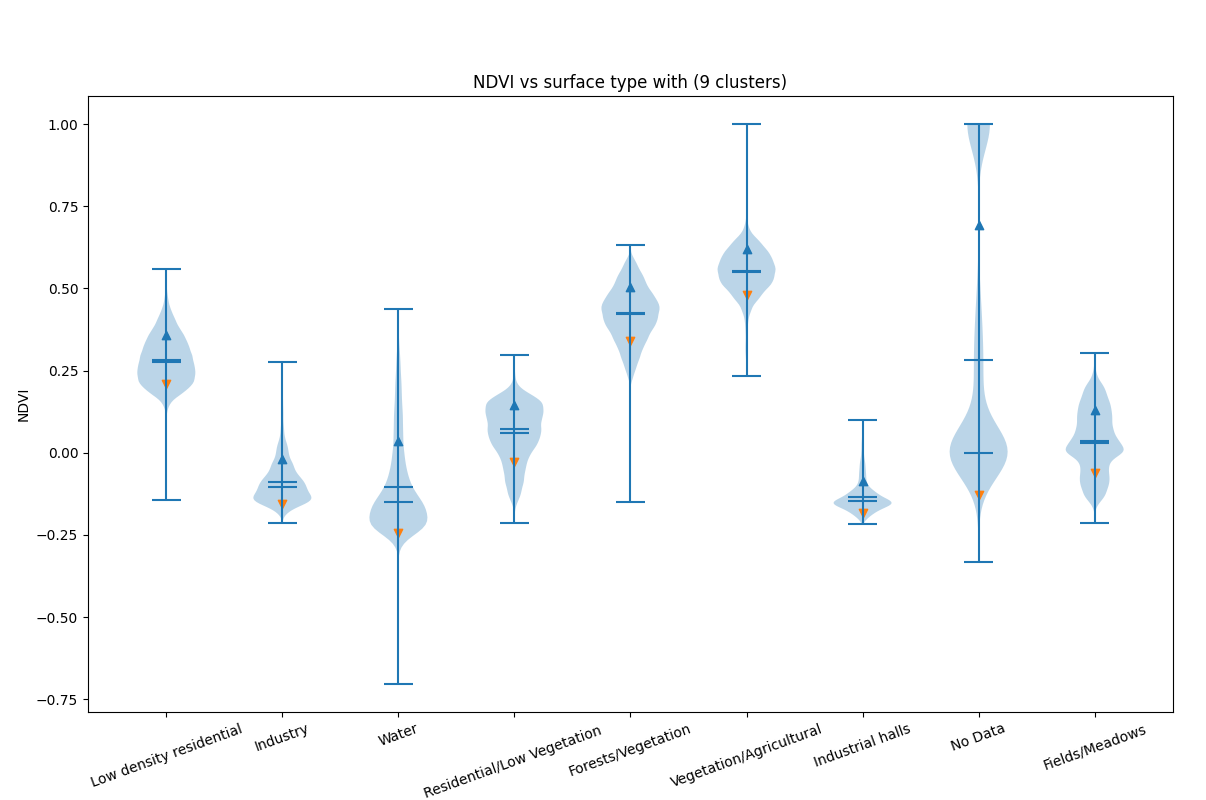
\includegraphics[width=\textwidth]{img/NDVIvsTypes.png}
%    \subcaption{Surface types and \ac{NDVI} value of associated pixels\label{fig:ndviVsTypes}}
%    \end{subfigure}
%    \caption{Correlation analysis of Bremen Landsat 8 Data\label{fig:uhidetecion}}
%\end{figure}
% summery of above 
%
\section{Discussion}
The pipeline approach works quite well with different data sources and areas, to gain insides and analysis data quickly.
The use of level 1 data to find \acp{UHI} based on temperature differentials allows to analyse real time data from the satellites that is less then a week old, while the level 2 \ac{LST} is made available a few weeks after the acquisition.
The extend of the detected \acp{UHI} varied between the processing levels while the affected areas remained the same. 
The processing steps should be improve to allow a higher similarity between the data levels, preprocessing of the data could eradicate outliers observed in the data sets (e.g.~the zero value in the industry hall class in \cref{fig:ndviVsLst}).
Another verification approach should be implemented to verify the classification e.g.~the Sentinel-2 land cover data. 
For further analysis especially when comparing cities a way must be found to define the \acp{UHI} by another metric then the mean temperature of the picture since the shape and urban composition as well as area selection influences the \ac{UHI} detection. 
%
%
This can be optimized by not only take the statistical average temperature of the image as baseline but include the surface type classification to include only the temperature of the urban areas.  
% 
%- Having a pipeline that can detect \ac{UHI} formation from different satellite or areal images, allows to track susceptibility of cities to \ac{UHI}, the data is widely available and the \ac{UHI} are detected independently from surface types (mostly)
%- long data archive allows time series of \ac{UHI} changes (depending on image quality and frequency) 
%
%- further studies could be done of estimating/modelling \ac{UHI} based on air temperature data from nearby stations, allowing modeling of \ac{UHI} near real time (identification of other factors (dryness, season, wind, weather etc. needs to be done)). 
%
%- Further investigation in the impact of Urban Cannopy and wind structures using edge detection and classification into "wind schlucht anfälligkeit"
%- Impact of \acp{UHI} to air pollution and surface ozone 
%
\section{Conclusions and Outlook}\label{sec:conclusio}
%
Urban planning is tasked in the coming decades with increasing the mitigation and resilience of heat effects, increased flood risk due to extreme weather and other climate change related effects on cities. 
This requires a deep understanding and investigation of the underling phenomenons. 
Out of these insights technical and policy decisions need to be made, to protects inhabitants from the negative effects of the changing conditions. \\
%
Many of the possible solutions against one effect have an positive effect on other climate related urban phenomenons.
Floodplains or natural wet vegetated areas within a city reduce temperature due to latent heat conversion and flood resistance due to higher water storage capacity of the city area and reduction of water ways. Trees reduce temperature and slow airflow within long and narrow streets.\\ 
In many cases only a few options are possible to implement due to geographic factors, construction area or budget limitations. 
To choose the most effective solutions the impact of possible options have to be known and compared. 
The development of tools, to allow quick analysis and measure the impact of implemented decisions, is one the steps in the needed courses of action.
Remote sensing data, is an available, low cost and quick way to get an overview and possible areas to implement countermeasures. 
The implemented pipeline with python allows the use of two current and past earth observation satellite systems (Landsat 8 and Landsat 7) to analyse the current and past development of \acp{UHI}, aid decisions and judge the impact of implemented counter measures.
While the implemented solution proposed in this far from feature complete it could serve as the base for further research and development as part of a tool set for scientists, policy makers and urban planners. 
\newpage
\printbibliography
\end{document}

%The surface classes where correlated with the %TODO check 
%Kataster data from Bremen as well as with OSM data. % todo do 
%
%Ziel Projekt teil: 
%- detection and error margins in \ac{UHI} detection using remote sensing data 
%- data pipeline to create maps of \ac{UHI} in areas 
%- surface classification based on remote sensing data correlated with 2nd and 3rd sources (kataster/ OSM) 
%- \ac{UHI} "cores" identification 
%
%Master Fragestellungen: 
%- Correlation zw. \ac{UHI} und Pollutants? 
%https://pubs.acs.org/doi/epdf/10.1021/cr5006815 
%- Real time \ac{UHI} size/occurrence prediction based on ground temperature stations (Bremen Airport) and pollutant levels? 
%- \ac{UHI} classification in different environments, causes and effects, mitigation stategies? (e.g. Classification of Surface types, vegetation etc. within different climate zones (Phoenix, Bremen, Karlruhe, Essen, Something meditareiean, Afrika (coastal, arid, etc) /paper with adis abbeba)
%
%\subsection{}

%Of the different bands available from the used satellite data (Landsat7 and Landsat8), 
%the visible and near infrared bands where used for clustering. 
%The clustering was done using the simple k-means algorithm. 
%Different configuration where used %todo add pictures? 
%These where compared and referenced with ground truth data %todo add error and limitations refgerenec here 


